% ================================================
% =                 EXPERIMENTS                  = 
% ================================================ 

This section includes all experiments carried out for evaluating the difference between the two approaches considered in the BEV2Seg\_2 pipeline, experiments to study what is the influence of extrinsic parameters modification as data augmentation technique for semantic segmentation of BEV images and the final evaluation of the proposed annotation pipeline of occupancy, occlusion and driveable areas.

\subsection{BEV2Seg\_2}

Both approaches, segmenting-then-IPM and IPM-then-segmenting, were trained under the same conditions. During fine-tuning for the segmentation task, encoder layers were left unfrozen, allowing the entire model to adapt to the training data. Input images were preprocessed using the \textit{SegformerImageProcessor}, which includes resizing to $512 \times 512$ pixels, rescaling pixel values by a factor of $1/255$, and normalizing with ImageNet mean and standard deviation values~\cite{imagenet}. This preprocessing step ensures the input format is consistent with what the pretrained encoders expect.

Semantic masks were provided during training with the \texttt{reduce\_labels} parameter set to \texttt{False}, as the dataset includes a "background" class. This configuration ensures that all pixel classes, including background, contribute to gradient computation during optimization. All experiments were executed on the hardware setup described in Table~\ref{tab:hardware}. From the six available Segformer encoder variants, three were selected for evaluation: MiT-b0, MiT-b2, and MiT-b4. Due to its larger size, the MiT-b4 model required two gradient accumulation steps to fit within the GPU's memory constraints. Checkpoints were saved based on evaluation loss, a design decision made despite ongoing discussions about whether loss or mean intersection over union is the better metric for model selection. A basic linear learning rate scheduler was applied throughout training and the loss function employed was \texttt{BCEWithLogitsLoss}, which is well-suited for multi-label semantic segmentation tasks, as it combines sigmoid activation and binary cross-entropy in a numerically stable way following the Segformer implementation.

\hl{Complete this table.}
\begin{table}[h]
    \centering
    \begin{tabular}{c l c}
        \toprule
        \textbf{Component} & \textbf{Specifications} & \textbf{Num workers} \\
        \midrule
        CPU         & - & 8 \\
        GPU         & - & 2 \\      
        Memmory     & - & - \\
        OS          & - & - \\
        \bottomrule
    \end{tabular}
    \caption{ Hardware used for experiments }
    \label{tab:hardware}
\end{table}

Regarding to the used notation, the models that follow the segment-then-IPM pipeline to obtain BEV semantic masks are referred to as \texttt{raw2seg\_bev}, while those that first apply IPM and then perform segmentation are named \texttt{raw2bev\_seg}.

The two approaches were firstly trained using the smallest Segformer model variant, MiT-b0, for $20.7K$ steps without applying any regularization technique. This initial experiment was performed to observe whether the models were able to learn and predict on the dataset and see if them suffered from overfitting. Also, for this purpose, the choice of MiT-b0 was intentional as it trains faster and, due to its limited capacity, is less prone to extreme overfitting compared to larger models. This made it a suitable candidate for testing different hyperparameter configurations in a lightweight environment.

\begin{figure}[h!]
    \centering
    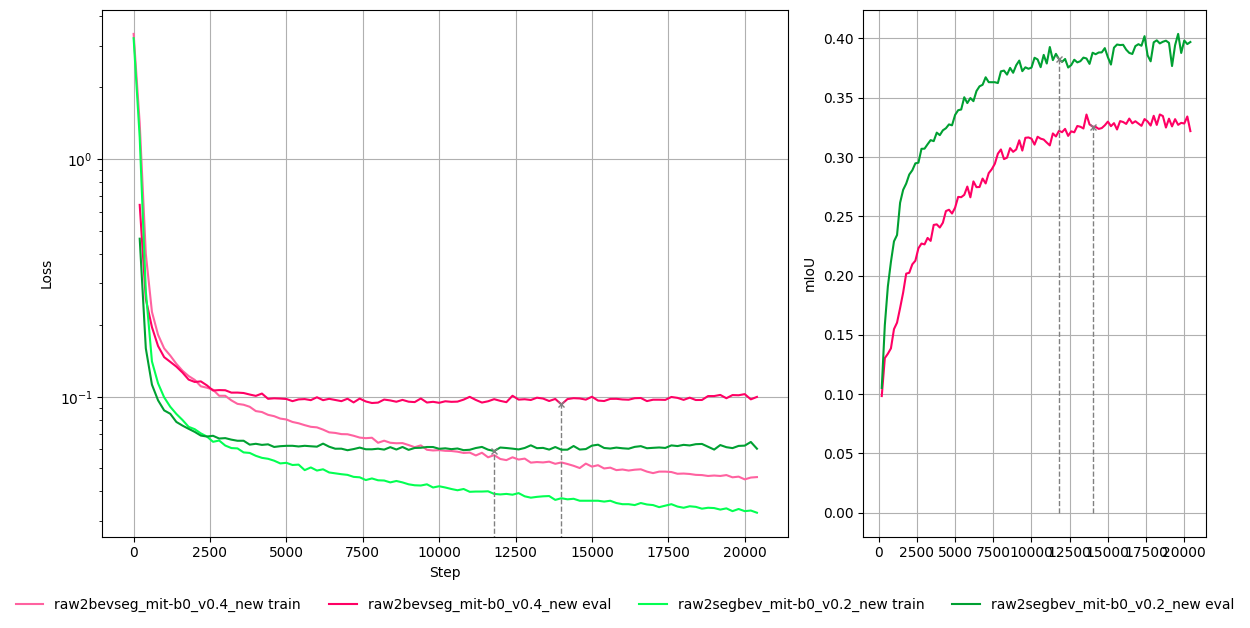
\includegraphics[width=0.7\linewidth]{./images/experiments/overfitting_bev_nu.png}
    \caption{Training and evaluation loss of raw2seg\_bev and raw2bev\_seg MiT-b0 models without any regularization technique}
    \label{fig:overfitting_mit-b0}
\end{figure}

As shown in Figure~\ref{fig:overfitting_mit-b0}, both models showed clear signs of overfitting. While the training loss continued to decrease continuously, the validation loss began to increase, indicating a lack of generalization and failure to converge. These results highlight the importance of introducing regularization techniques even for small model sizes. Additionally, no signs of exploding gradients were observed during the training of these models. 

Two main approaches were selected to tackle the overfitting problem: weight decay (also known as L2 regularization) and data augmentation. Weight decay penalizes large weights during training, and makes the model more robust and less prone to memorizing irrelevant details; while data augmentation techniques introduces variability in the training dataset enabling the model to adapt better to unseen data. However, the introduction of data augmentation techniques into \aclink{BEV} images domain is not trivial and raises another research question.

It is also important to highlight the difference in metrics between the two models. Even though the backbone and training hyperparameters remain the same, there is a noticeable difference in both the loss values and the \aclink{mIoU} between the models. This difference is primarily due to the fact that the evaluation datasets differ. Specifically, the approach that segments the image first and then reprojects it is evaluated using semantic masks in the camera view, while the approach that first reprojects images into \aclink{BEV} and then performs segmentation is evaluated using masks directly in the \aclink{BEV} domain.

This distinction motivates the analysis shown in Figure~\ref{fig:normal_vs_bev_evaluation}, where the model \texttt{raw2segbev\_mit-b0\_v0.3} is evaluated on the test set twice: once using semantic masks in the camera domain and once using \aclink{BEV} masks. The figure displays the per-class \aclink{mIoU} for all the semantic categories the model was trained on, and two main observations emerge.

\begin{figure}[h!]
    \centering
    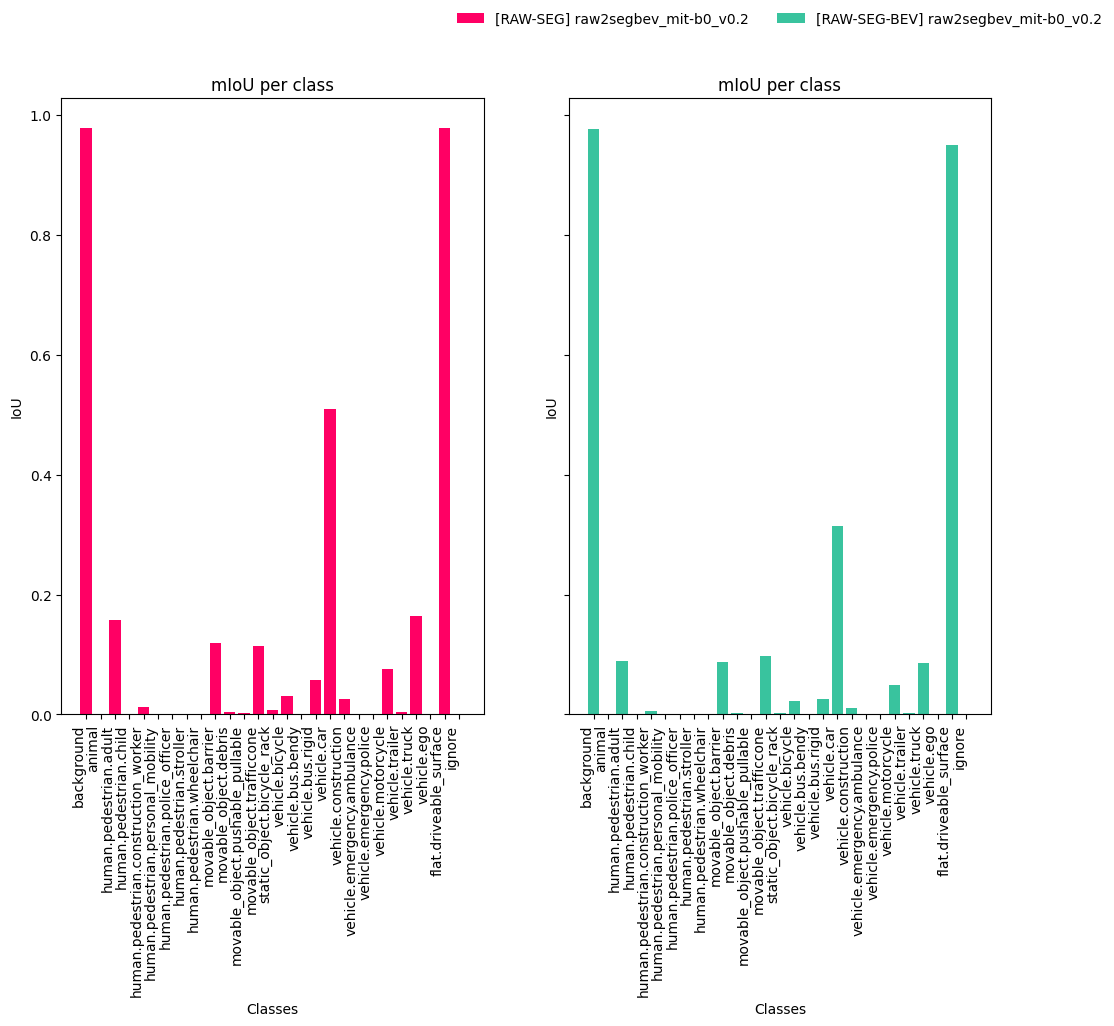
\includegraphics[width=0.8\linewidth]{./images/experiments/raw2segbev_mit-b0_v0.2_test_evaluation.png}
    \caption{Model evaluated with normal and BEV images}
    \label{fig:normal_vs_bev_evaluation}
\end{figure}

First, there's a clear imbalance in performance between dominant classes such as \texttt{background} and \texttt{flat.driveable\_area}, and the remaining, less frequent classes. Many of the minority classes show extremely low or even zero \aclink{IoU} scores. This is partly due to the inherent class imbalance in the dataset: some semantic classes have no annotated pixels at all (see Appendix~\ref{appendix:OLDatasets} for more details).

Second, all metrics are significantly higher when the model is evaluated using standard camera-domain masks. Reprojecting the masks to BEV introduces several effects: (1) a fixed background area appears in the BEV space that lies outside the camera's field of view; (2) the maximum scene distance is reduced to 15 meters (see reprojection parameters in Section~\ref{sec:bev2seg_2}), which limits the presence of distant objects: minority classes like pedestrians are often excluded unless they are very close to the vehicle, while driveable areas and vehicles dominate the scene; and (3) the resolution is reduced to $1024 \times 1024$ pixels.

All these factors lead to a lower total number of pixels in the BEV dataset. As a result, each misclassified pixel has a greater impact on the overall evaluation, making errors more costly and consequently lowering the average performance metrics.

To address this, many training methods use class weighting in the loss function to penalize misclassifications of minority classes more heavily than those of majority classes. However, in this particular project, it is not essential to maintain all class distinctions provided by the dataset. Therefore, we investigate whether merging semantic classes can help mitigate the effects of class imbalance.

With all of this in place, the training strategy is designed to support experimentation in order to answer three main research questions:

\begin{itemize}
    \item \textit{Does the label's merging strategy helps increasing the model's performance on the low presence classes?}
    \item \textit{Which data augmentation technique is more effective for trainig a model directly on \aclink{BEV} images on a semantic segmentation task?}
    \item \textit{Which of the two approaches performs better for BEV driveable area segmentation?}
\end{itemize}

\hl{Mention the used hyperparameters for training the models.}

\subsubsection{Merging labels}
As previously discussed, to improve model performance on the dataset’s minority classes, a semantic label merging strategy was applied. This approach combines less represented semantic classes into more general, representative categories. Notably, this same merging strategy was already used in the annotation pipeline, so it was incorporated during training using the same look-up table of merging rules described in Table 3. The training and evaluation scripts were adapted accordingly to apply the merging rules consistently.

Table~\ref{tab:merging_comparison_bev} shows the results of two models evaluated on the same test set using \aclink{BEV} masks. Model A was trained using the full set of original semantic classes, while Model B was trained using the merged classes, thereby reducing the total number of labels. 

Despite this, in general the results indicate that in some specific classes, Model A achieves a higher \aclink{IoU}; however, in those same cases, Model B tends to maintain a similar or slightly better F1-score. The most notable improvement is observed in the \texttt{vehicle.car} class, where the merging strategy significantly boosts model performance. Nevertheless, the overall results reveal that while Model A achieves higher \aclink{IoU} scores in certain individual classes, Model B often maintains comparable or even slightly superior F1-scores in those same cases.

The fact that the model with merged labels achieves equal or better mean F1-scores (mF1), even when its mean \aclink{IoU} is lower, suggests that simplifying the semantic space does not decrease the model’s ability to identify important instances. Instead, it reduces the penalty from underrepresented classes. Additionally, by reducing the number of classes, the overall average of the metrics improves, as it avoids dilution from irrelevant or sparsely populated classes. This makes label merging especially useful in cases where fine-grained segmentation isn’t necessary, and consistency across the whole model is more important.

\begin{table}[h!]
    \centering
    \tiny
    \begin{tabular}{llcccc}
    \toprule
    \textbf{Merged Class} & \textbf{Original Label} & \textbf{mIoU A} & \textbf{mIoU B} & \textbf{mF1 A} & \textbf{mF1 B} \\
    \midrule
    background & background & 0.98 & 0.97 & 0.99 & 0.99 \\
    \midrule
    animal & animal & 0.00 & 0.00 & 0.00 & 0.00 \\
    \midrule
    human.pedestrian.adult & human.pedestrian.adult & 0.09 & 0.08 & 0.11 & 0.11 \\
     & human.pedestrian.child & 0.00 & - & 0.00 & - \\
     & human.pedestrian.construction\_worker & 0.01 & - & 0.01 & - \\
     & human.pedestrian.personal\_mobility & 0.00 & - & 0.00 & - \\
     & human.pedestrian.police\_officer & 0.00 & - & 0.00 & - \\
     & human.pedestrian.stroller & 0.00 & - & 0.00 & - \\
     & human.pedestrian.wheelchair & 0.00 & - & 0.00 & - \\
    \midrule
    movable\_object.barrier & movable\_object.barrier & 0.09 & 0.14 & 0.10 & 0.17 \\
     & movable\_object.debris & 0.00 & - & 0.00 & - \\
     & movable\_object.pushable\_pullable & 0.00 & - & 0.00 & - \\
     & movable\_object.trafficcone & 0.10 & - & 0.12 & - \\
     & static\_object.bicycle\_rack & 0.00 & - & 0.00 & - \\
    \midrule
    vehicle.car & vehicle.bus.bendy & 0.00 & - & 0.00 & - \\
     & vehicle.bus.rigid & 0.02 & - & 0.03 & - \\
     & vehicle.car & 0.31 & 0.38 & 0.34 & 0.42 \\
     & vehicle.construction & 0.01 & - & 0.01 & - \\
     & vehicle.emergency.ambulance & 0.00 & - & 0.00 & - \\
     & vehicle.emergency.police & 0.00 & - & 0.00 & - \\
     & vehicle.trailer & 0.00 & - & 0.00 & - \\
     & vehicle.truck & 0.09 & - & 0.10 & - \\
    \midrule
    vehicle.ego & vehicle.ego & 0.00 & 0.00 & 0.00 & 0.00 \\
    \midrule
    vehicle.motorcycle & vehicle.bicycle & 0.02 & - & 0.03 & - \\
     & vehicle.motorcycle & 0.05 & 0.06 & 0.06 & 0.07 \\
    \midrule
    flat.driveable\_surface & flat.driveable\_surface & 0.95 & 0.94 & 0.97 & 0.97 \\
    \midrule
     & & 0.10 & 0.32 & 0.11 & 0.34 \\
    \bottomrule
    \end{tabular}

    \caption{Per-class metric comparison between Model A and merged Model B evaluated in BEV images}
    \label{tab:merging_comparison_bev}
\end{table}



\subsubsection{Data augmentation}
Data augmentations are commonly used in deep learning models to mitigate overfitting during training and improve model generalization. There exists multiple types of data augmentation on the image domain: from pixel-based transformations, such as color space modifications, histogram equalization or filtering operations; to geometric transformations, including translations, rotations, shearings and homographies. These techniques have been widely applied in computer vision tasks and have shown to enhance model performance. However, performing data augmentation in \aclink{BEV} is not an easy task, as \aclink{IPM} images are already homographies of camera images, resulting in inherent distorsions.

Filtering operations can be applied to both standard and \aclink{BEV} images but geometric transformations were selected as the primary data augmentation method for camera domain images following the strategies employed in training the SegFormer model \cite{segformer}. Accordingly, random resizing, random cropping, and horizontal flipping were chosen as augmentation operations for perspective images.

Regarding \aclink{BEV} data augmentations, some multi-view methods implement strategies such as random flipping and random scaling, while others operate in the frequency domain \cite{HSDA}. However, these approaches apply augmentations to perspective images before the BEV transformation. Performing random cropping on a \aclink{BEV} image may lead to significant information loss, as large portions of the image may consist of unlabeled background data, potentially resulting in crops with insufficient information for effective training (Figure~\ref{fig:bev_cropping}). 

\begin{figure}[h]
    \centering
    % Row labels
    \setlength{\tabcolsep}{1pt}  % Reduce column padding
    \renewcommand{\arraystretch}{0.5}
    \begin{tabular}{c c c c c c c c}

        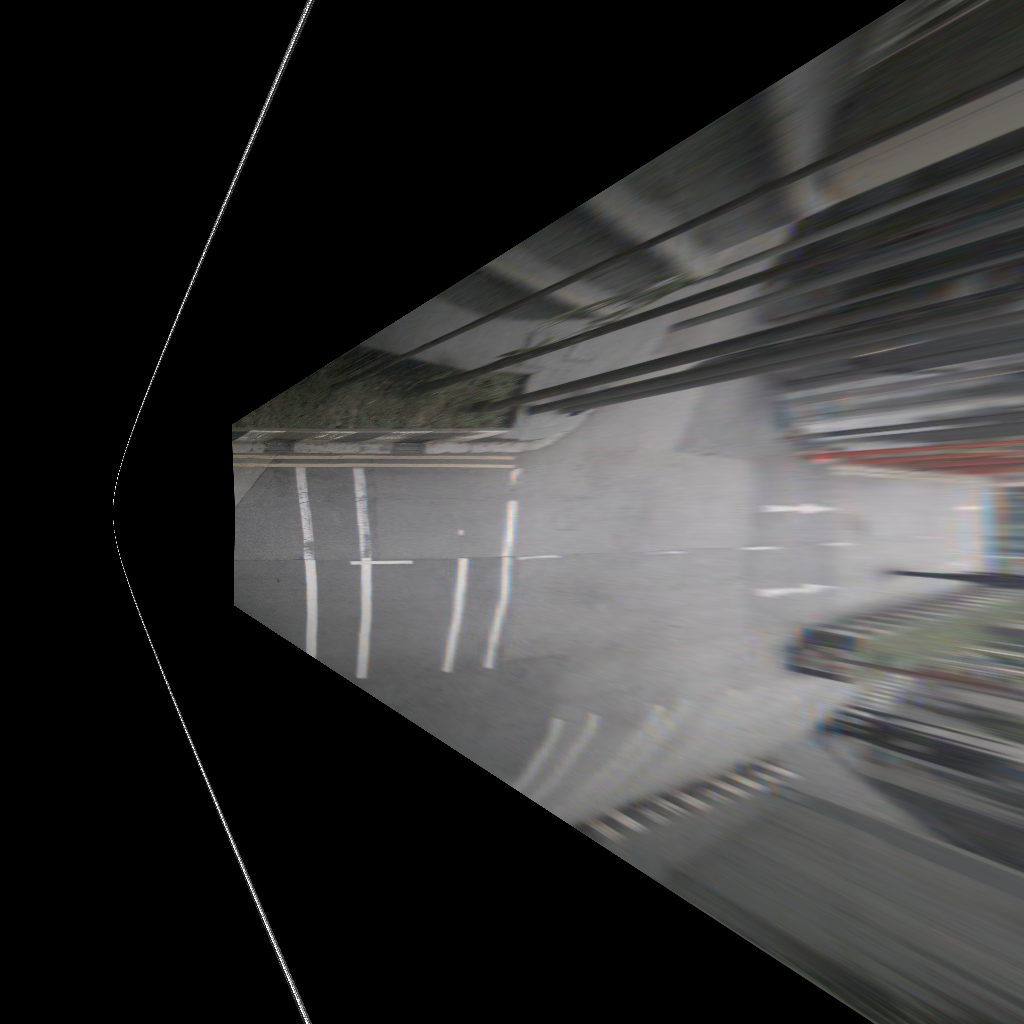
\includegraphics[width=0.12\textwidth]{images/methodology/mini/mini_0_bev.png} & 
        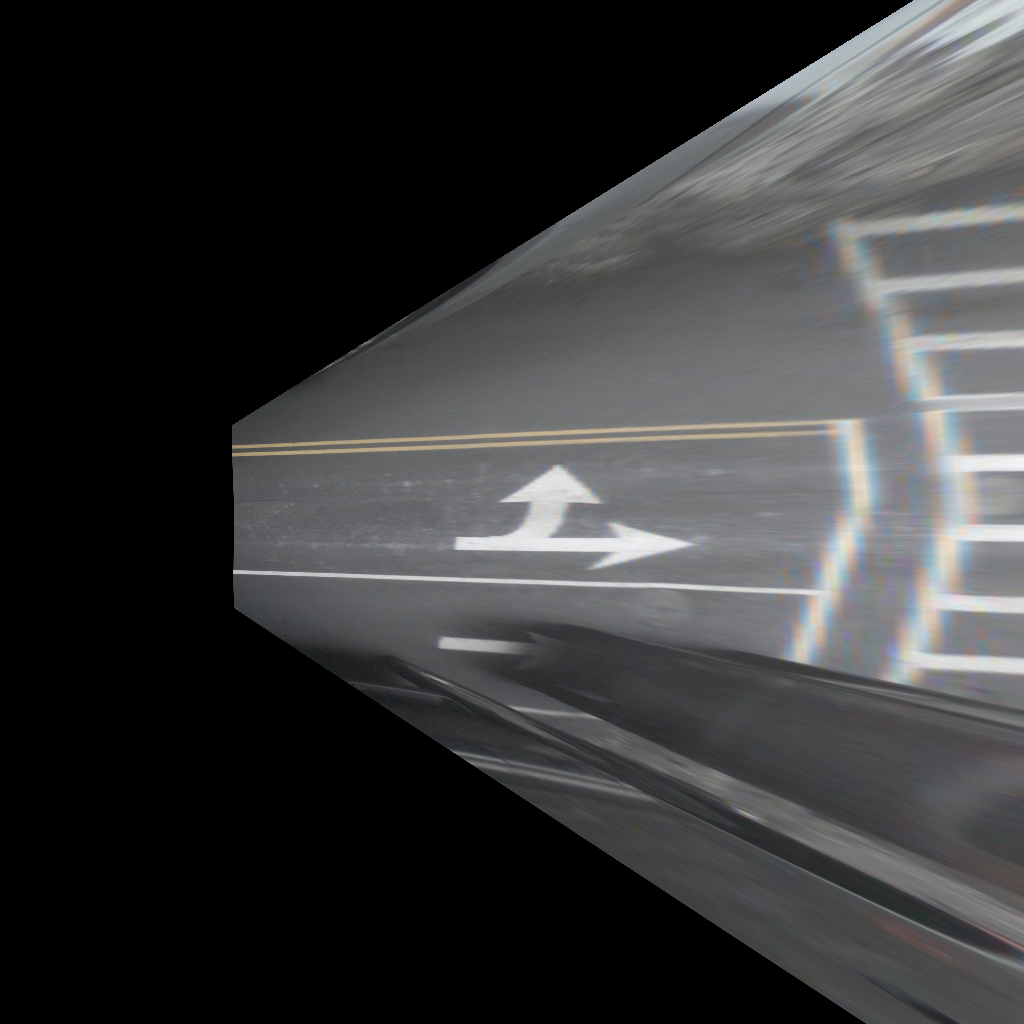
\includegraphics[width=0.12\textwidth]{images/methodology/mini/mini_1_bev.png} & 
        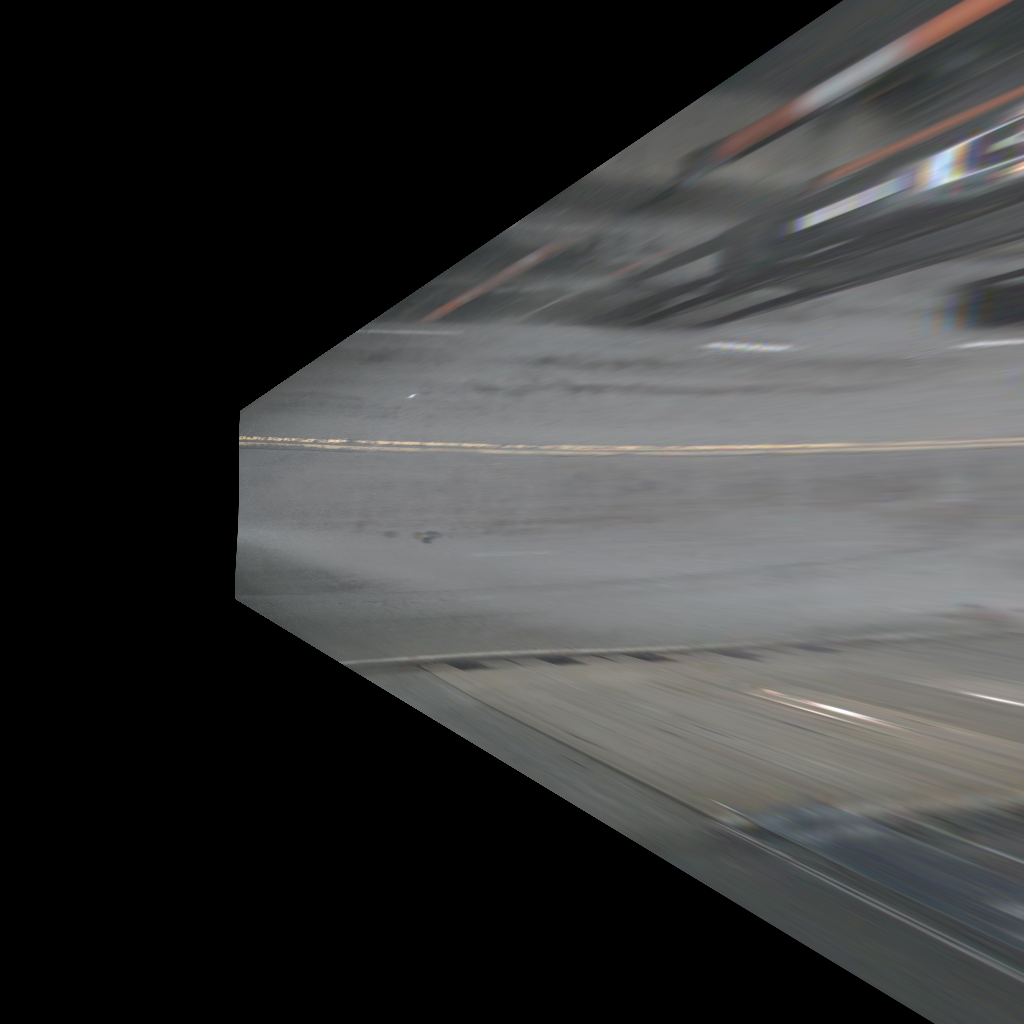
\includegraphics[width=0.12\textwidth]{images/methodology/mini/mini_2_bev.png} &
        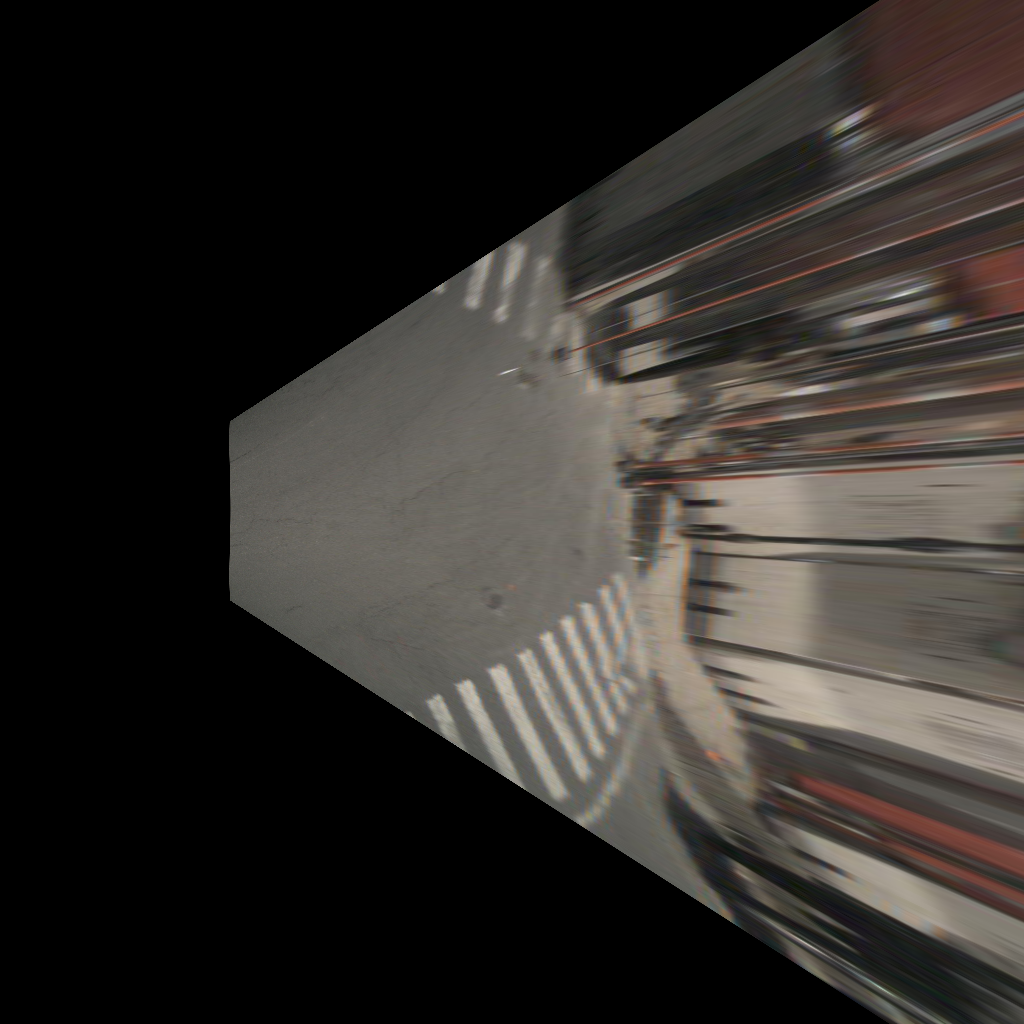
\includegraphics[width=0.12\textwidth]{images/methodology/mini/mini_3_bev.png} & 
        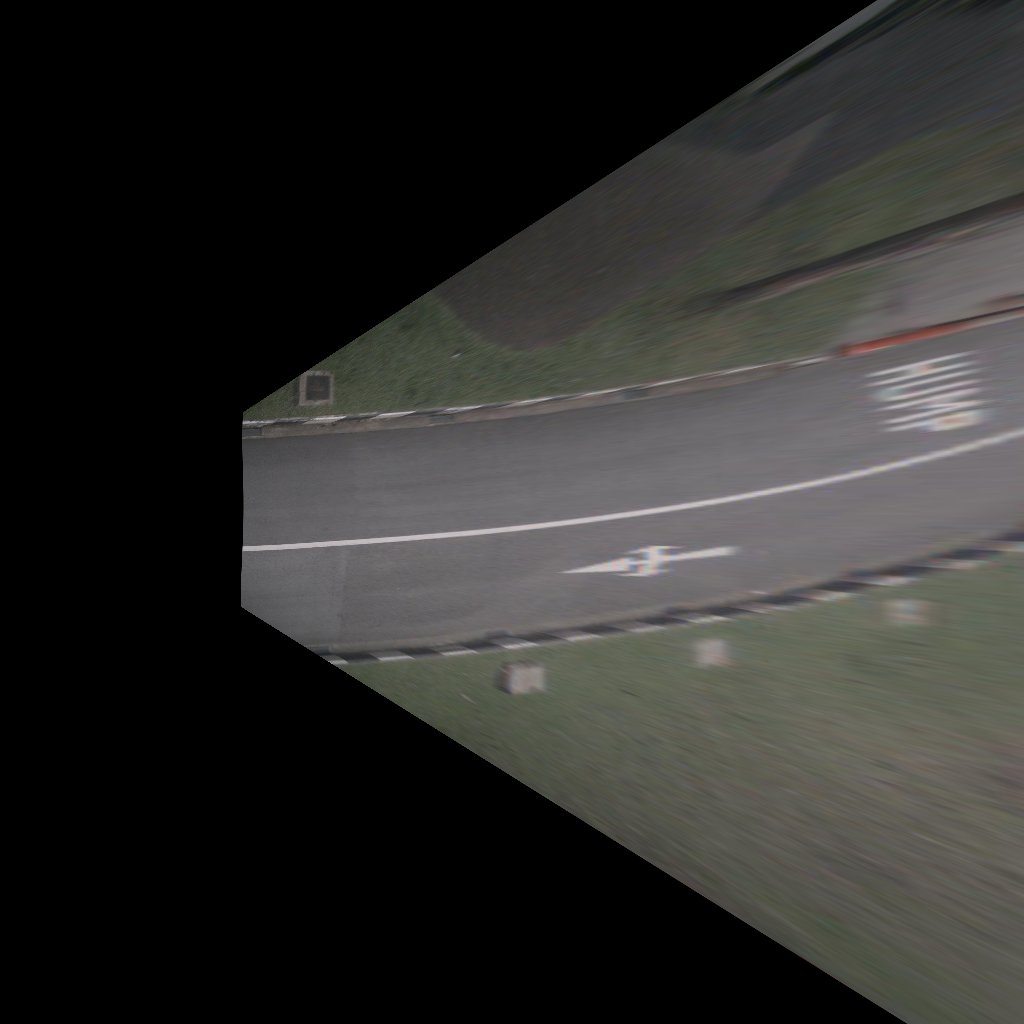
\includegraphics[width=0.12\textwidth]{images/methodology/mini/mini_4_bev.png} & 
        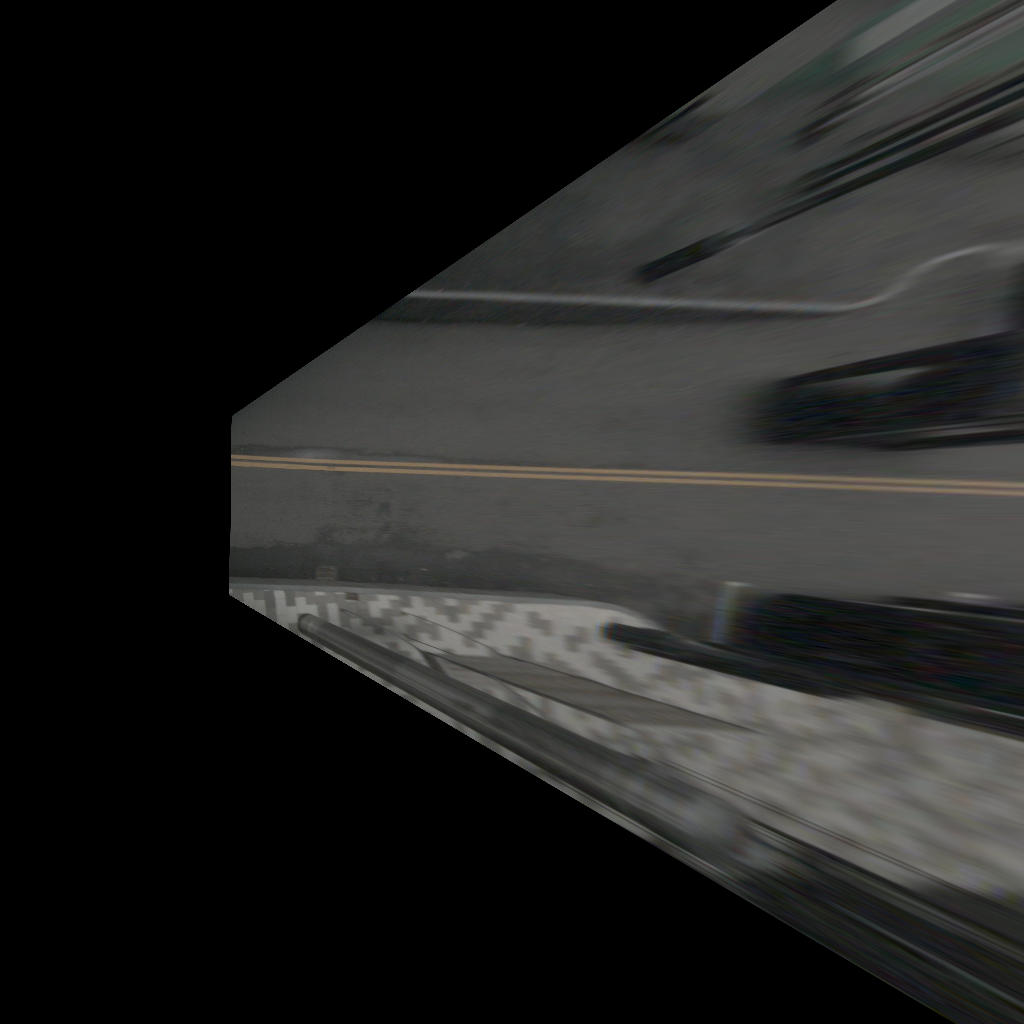
\includegraphics[width=0.12\textwidth]{images/methodology/mini/mini_5_bev.png} &
        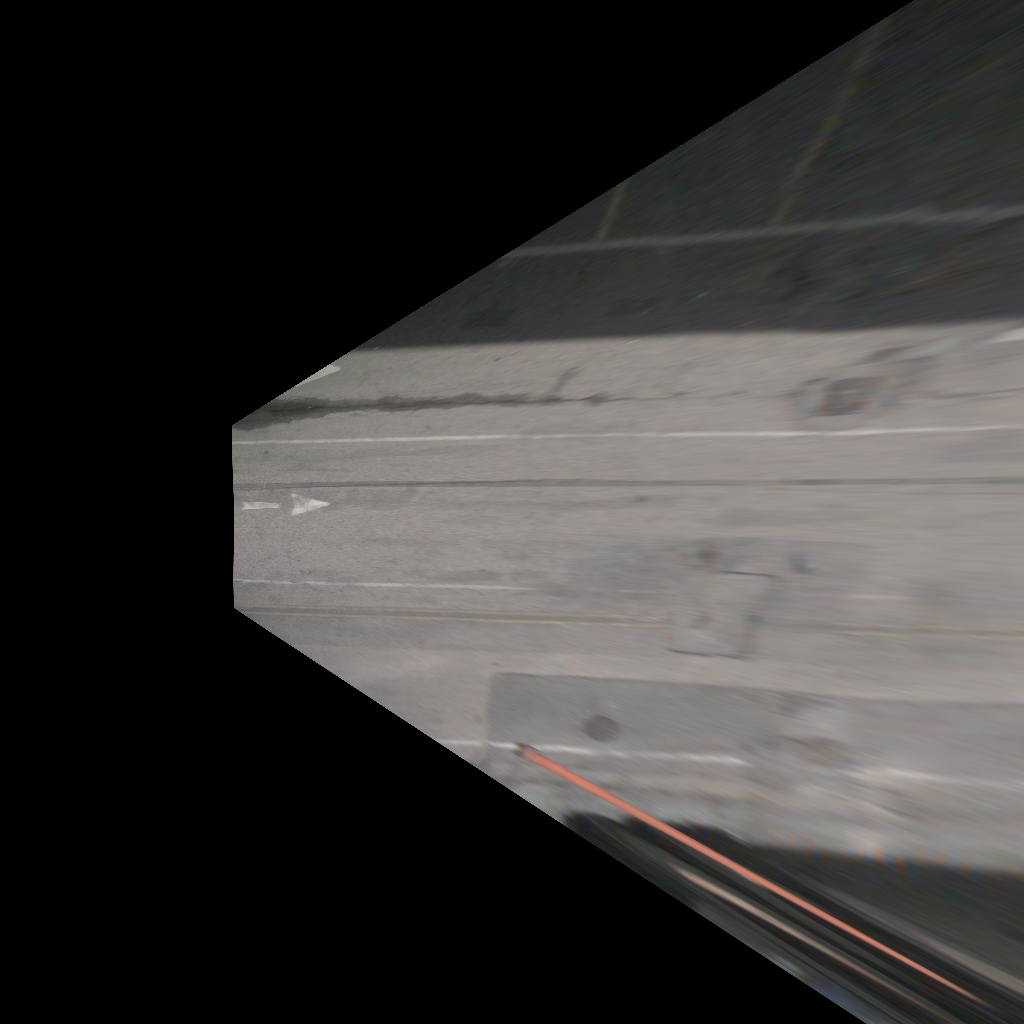
\includegraphics[width=0.12\textwidth]{images/methodology/mini/mini_6_bev.png} &
        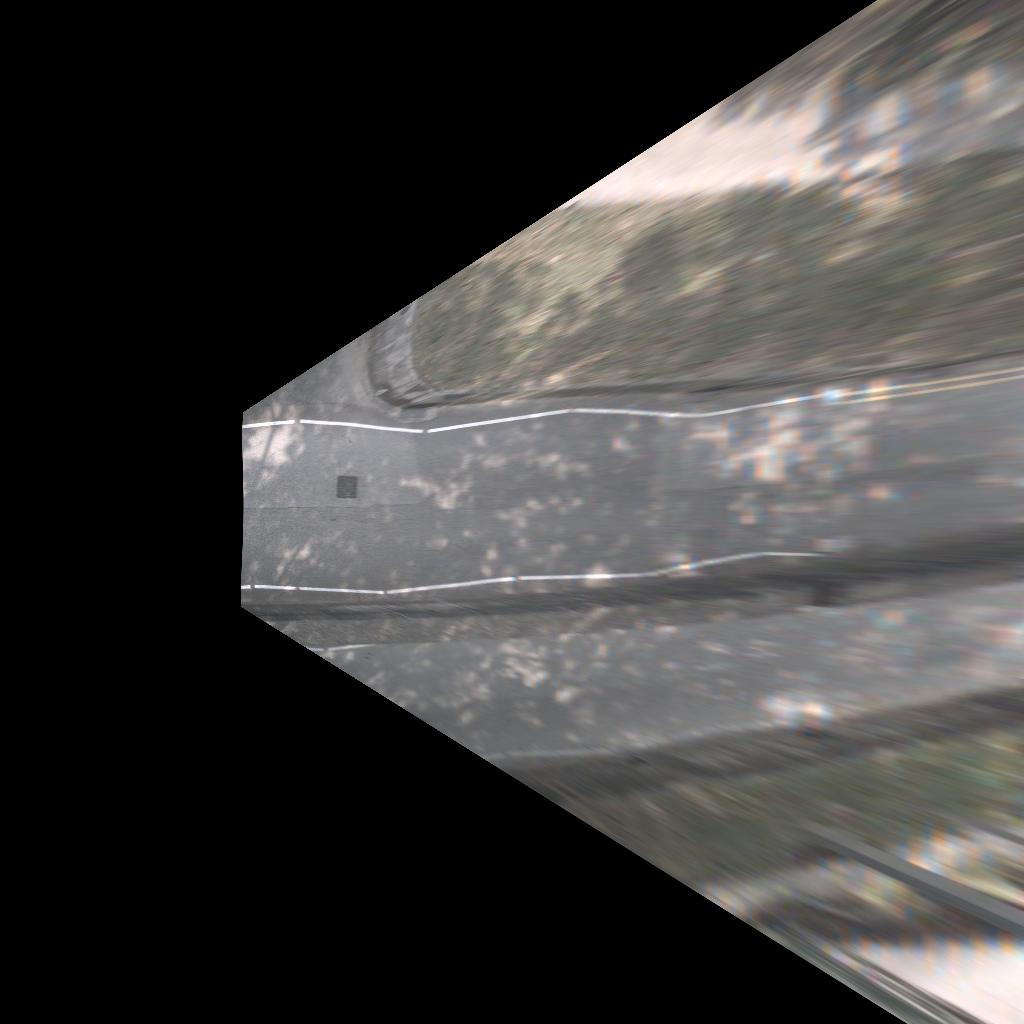
\includegraphics[width=0.12\textwidth]{images/methodology/mini/mini_7_bev.png} \\ 
        
        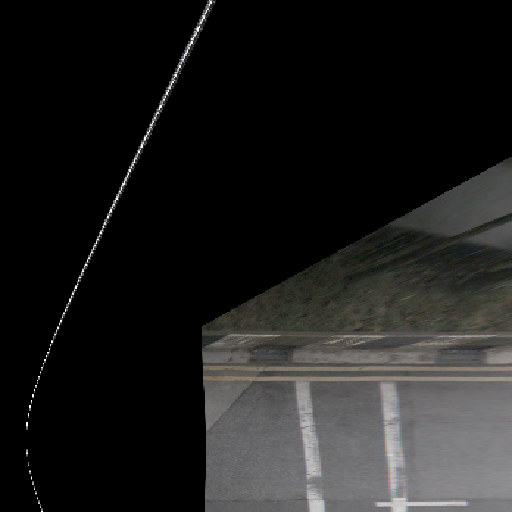
\includegraphics[width=0.12\textwidth]{images/methodology/data_augmentations/bev_crop_image_0_9.png} & 
        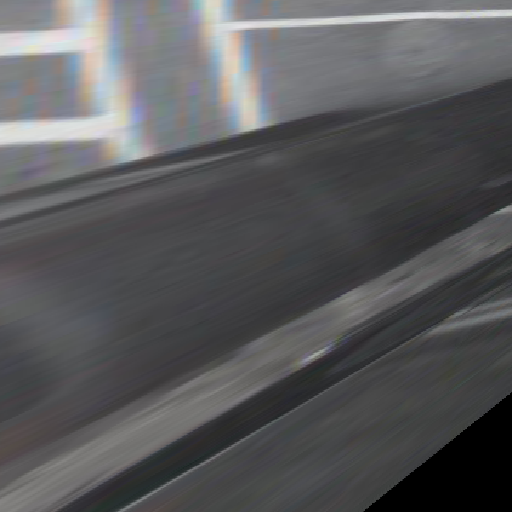
\includegraphics[width=0.12\textwidth]{images/methodology/data_augmentations/bev_crop_image_1_2.png} & 
        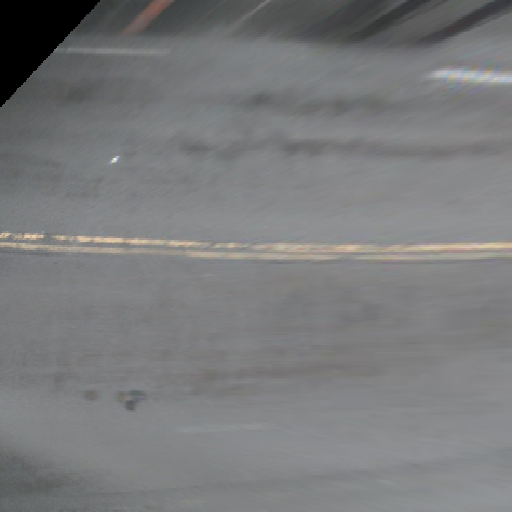
\includegraphics[width=0.12\textwidth]{images/methodology/data_augmentations/bev_crop_image_2_5.png} &
        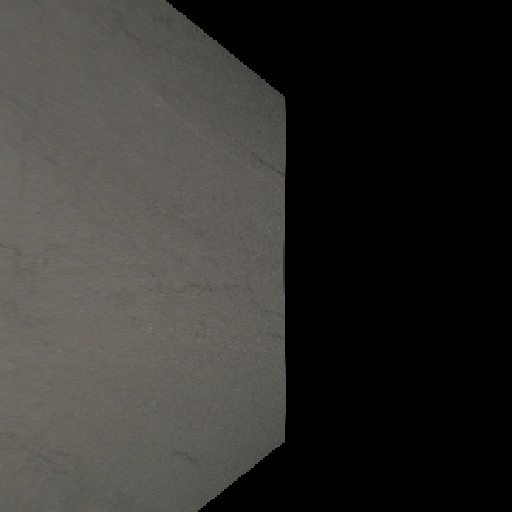
\includegraphics[width=0.12\textwidth]{images/methodology/data_augmentations/bev_crop_image_3_5.png} & 
        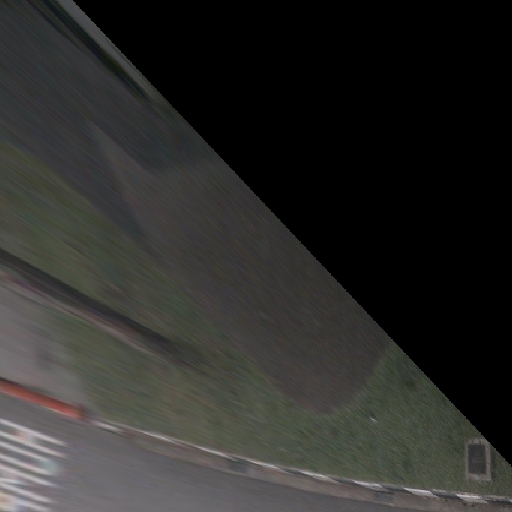
\includegraphics[width=0.12\textwidth]{images/methodology/data_augmentations/bev_crop_image_4_3.png} & 
        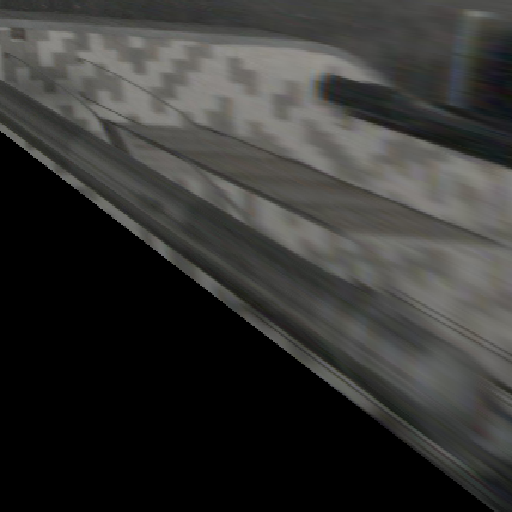
\includegraphics[width=0.12\textwidth]{images/methodology/data_augmentations/bev_crop_image_5_2.png} &
        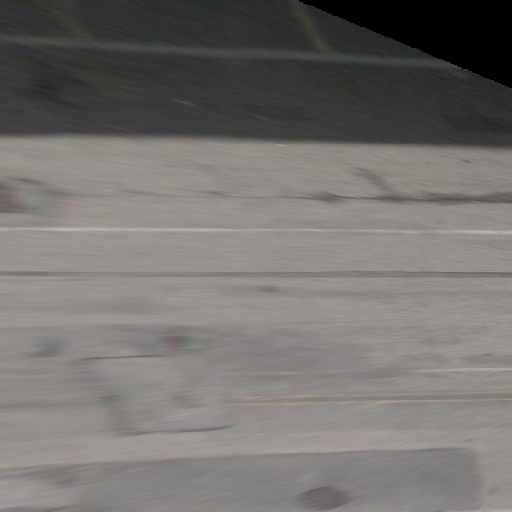
\includegraphics[width=0.12\textwidth]{images/methodology/data_augmentations/bev_crop_image_6_1.png} &
        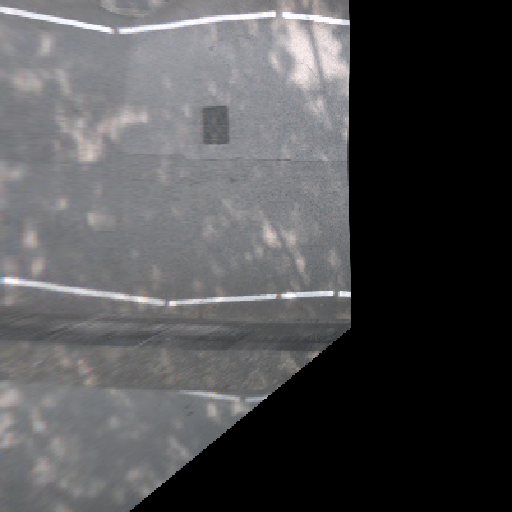
\includegraphics[width=0.12\textwidth]{images/methodology/data_augmentations/bev_crop_image_7_2.png} \\ 

        
\includegraphics[width=0.12\textwidth]{images/methodology/data_augmentations/bev_crop_mask_0_9.png} & 
        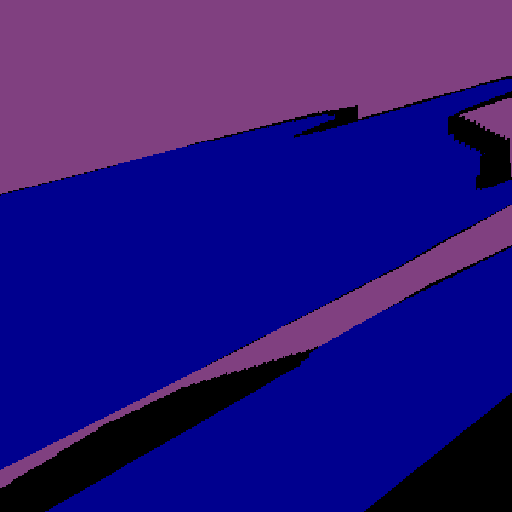
\includegraphics[width=0.12\textwidth]{images/methodology/data_augmentations/bev_crop_mask_1_2.png} & 
        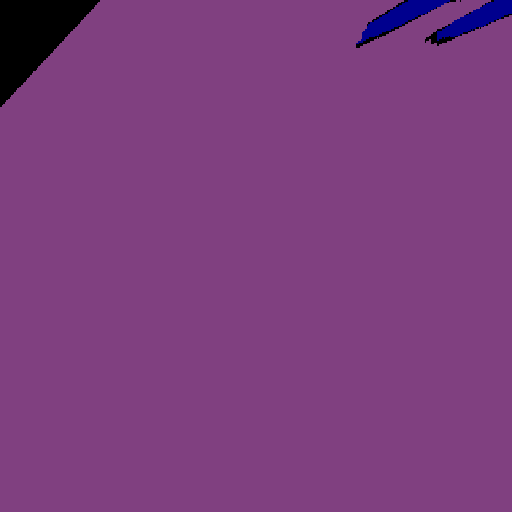
\includegraphics[width=0.12\textwidth]{images/methodology/data_augmentations/bev_crop_mask_2_5.png} &
        
\includegraphics[width=0.12\textwidth]{images/methodology/data_augmentations/bev_crop_mask_3_5.png} & 
        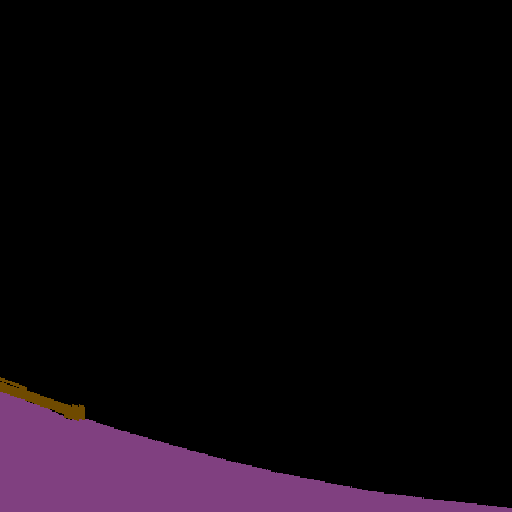
\includegraphics[width=0.12\textwidth]{images/methodology/data_augmentations/bev_crop_mask_4_3.png} & 
        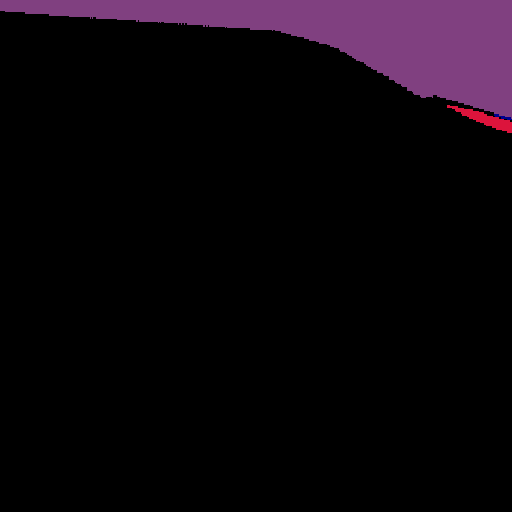
\includegraphics[width=0.12\textwidth]{images/methodology/data_augmentations/bev_crop_mask_5_2.png} &
        
\includegraphics[width=0.12\textwidth]{images/methodology/data_augmentations/bev_crop_mask_6_1.png} &
        
\includegraphics[width=0.12\textwidth]{images/methodology/data_augmentations/bev_crop_mask_7_2.png} \\

    \end{tabular}
    
    \caption{Random cropping and horizontal flipping on BEV images. Original BEV images on first row; random flipped and cropped images on second row and corresponding semantic masks on last row.}
    \label{fig:bev_cropping}
\end{figure}

In this context, a different approach was also considered: applying geometric transformations by modifying the camera's extrinsic parameters before reprojecting to \aclink{BEV} space. The objective is to introduce random transformations along one of the camera’s rotation axes, generating diverse \aclink{BEV} reprojections with varying degrees of distortion. This technique may enable the model to adapt to different extrinsic camera configurations, improving its robustness to variations in camera placement and orientation (Figure~\ref{fig:bev_data_aug}).

\begin{figure}[h]
    \centering
    % Row labels
    \setlength{\tabcolsep}{1pt}  % Reduce column padding
    \renewcommand{\arraystretch}{0.5}
    \begin{tabular}{c c c c c c}
        & $-0.25$ rad & $-0.125$ rad & $0.0$ rad & $0.125$ rad & $0.25$ rad \\ 
        
        \rotatebox{90}{\textbf{Yaw}} & 
        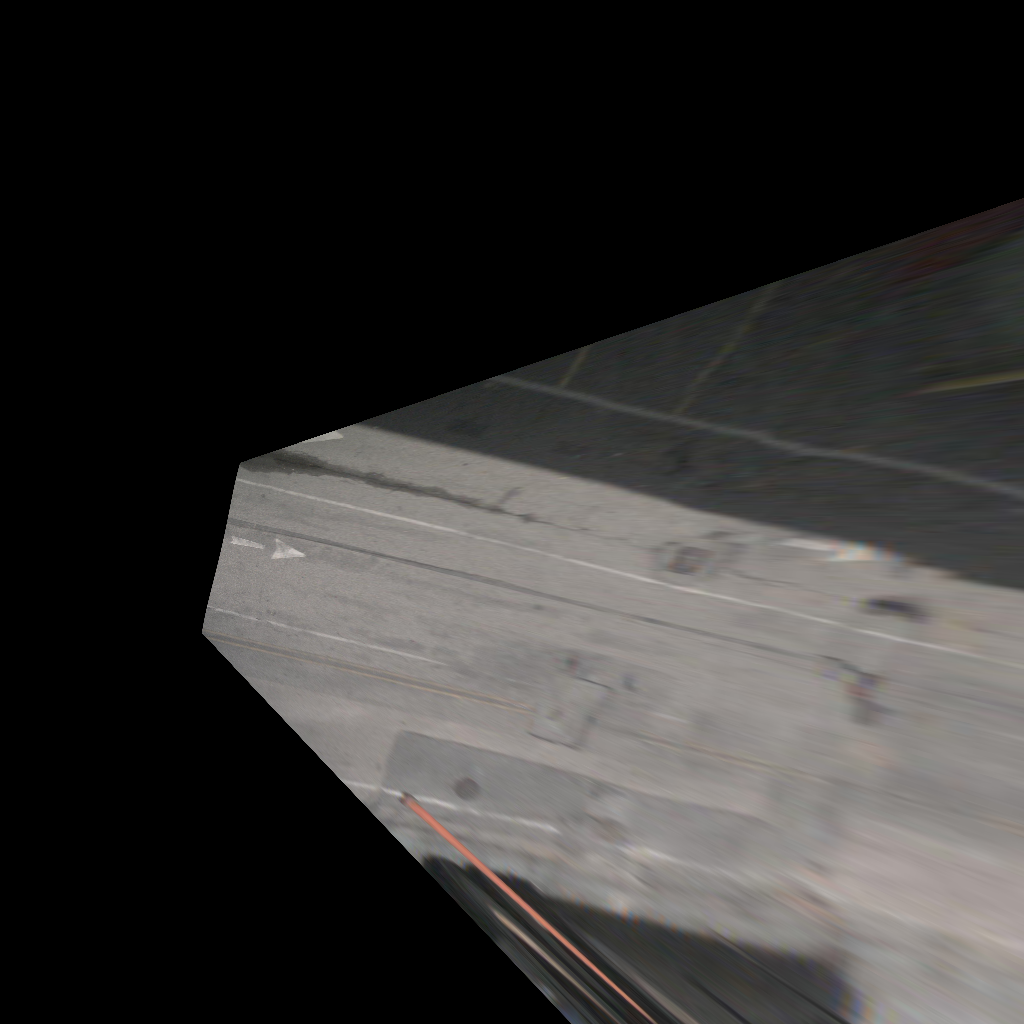
\includegraphics[width=0.15\textwidth]{images/methodology/data_augmentations/rx_-0.25_0.png} & 
        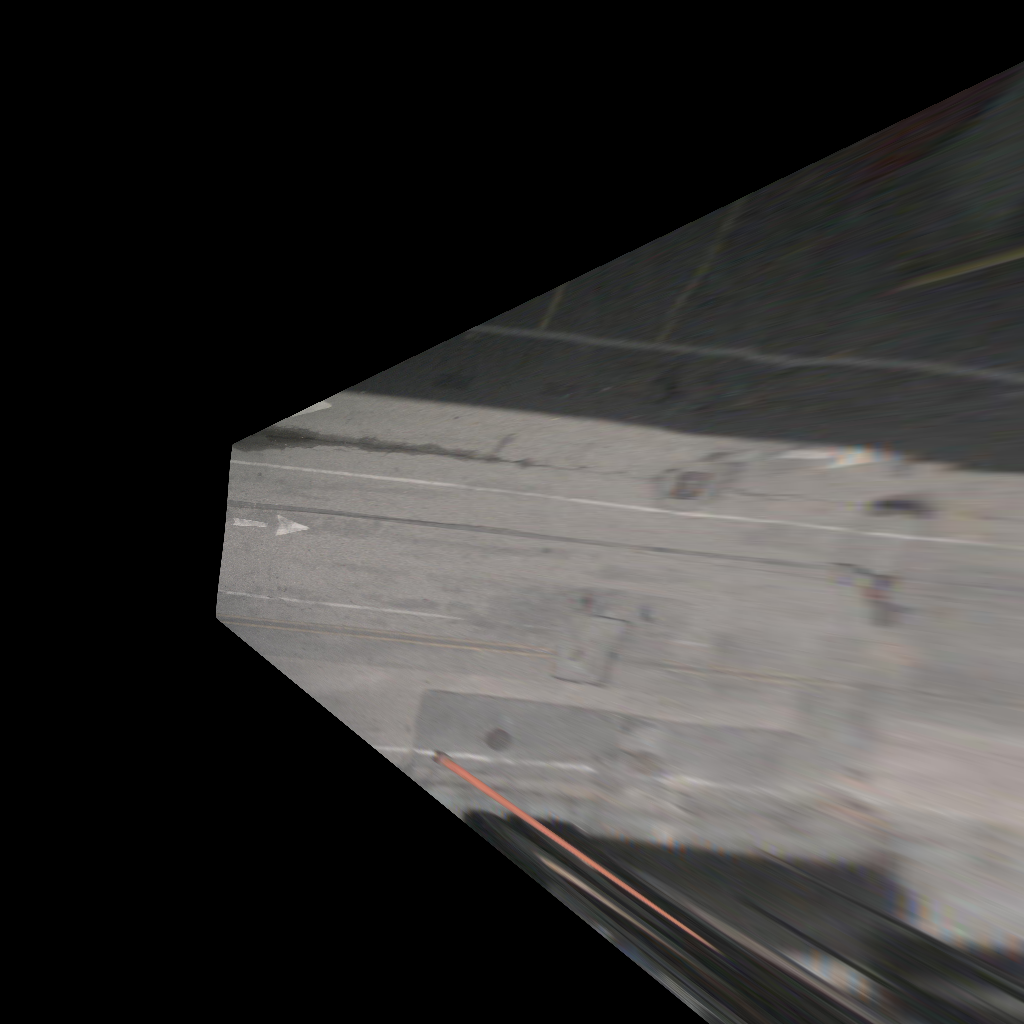
\includegraphics[width=0.15\textwidth]{images/methodology/data_augmentations/rx_-0.125_1.png} & 
        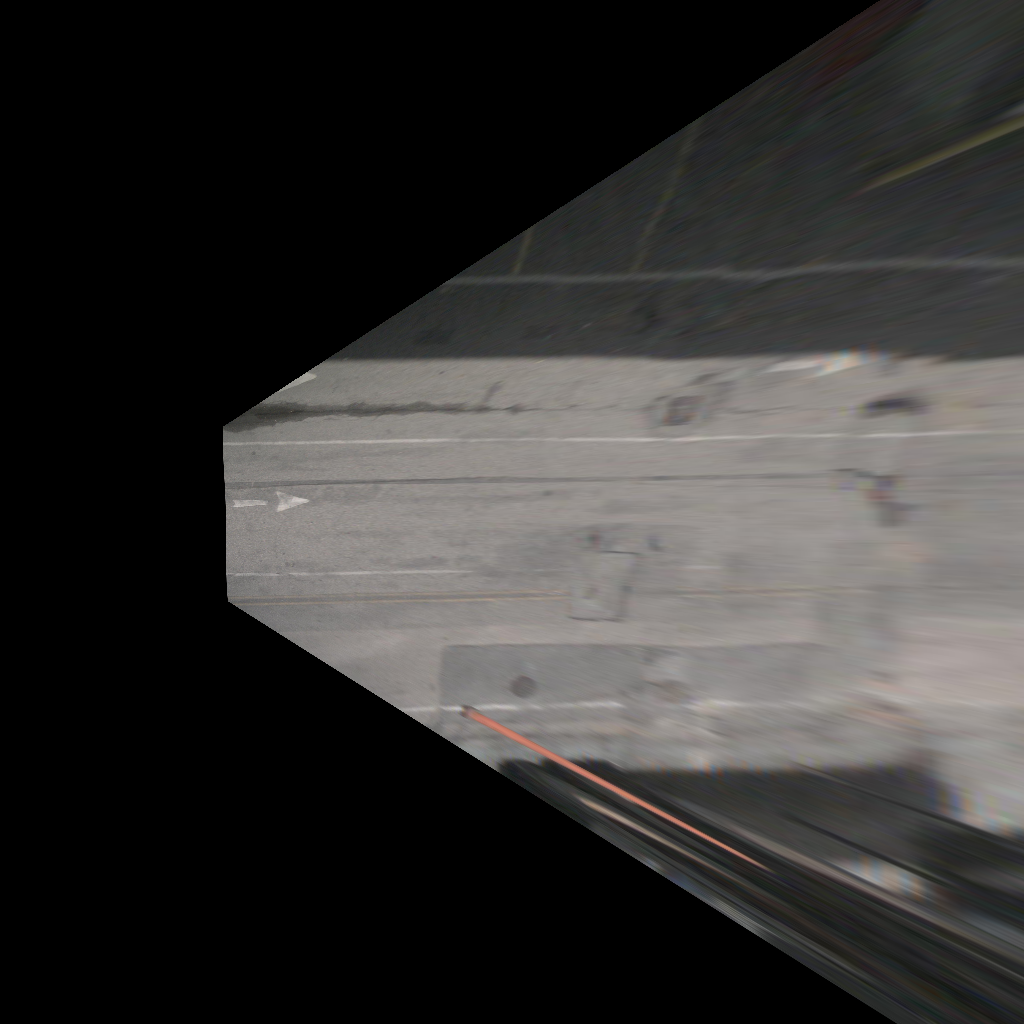
\includegraphics[width=0.15\textwidth]{images/methodology/data_augmentations/rx_0.0_2.png} & 
        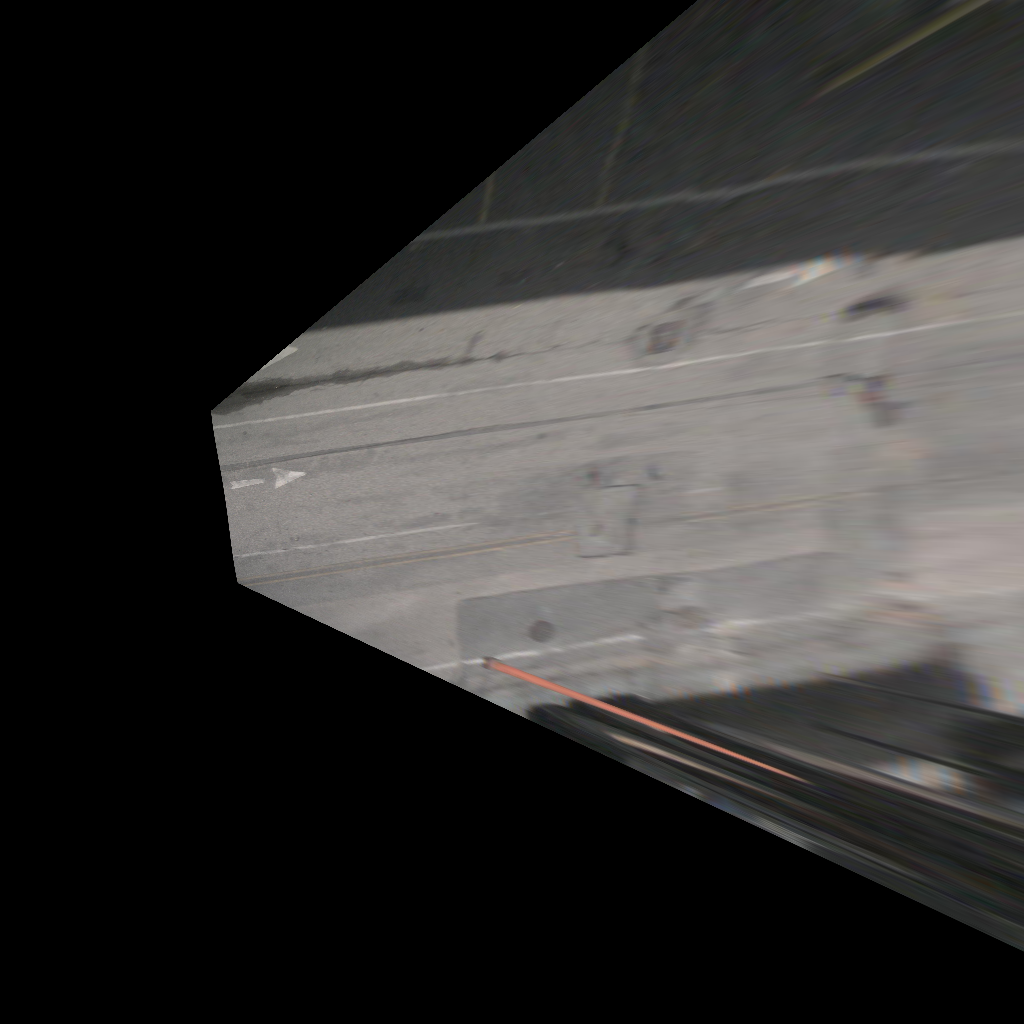
\includegraphics[width=0.15\textwidth]{images/methodology/data_augmentations/rx_0.125_3.png} & 
        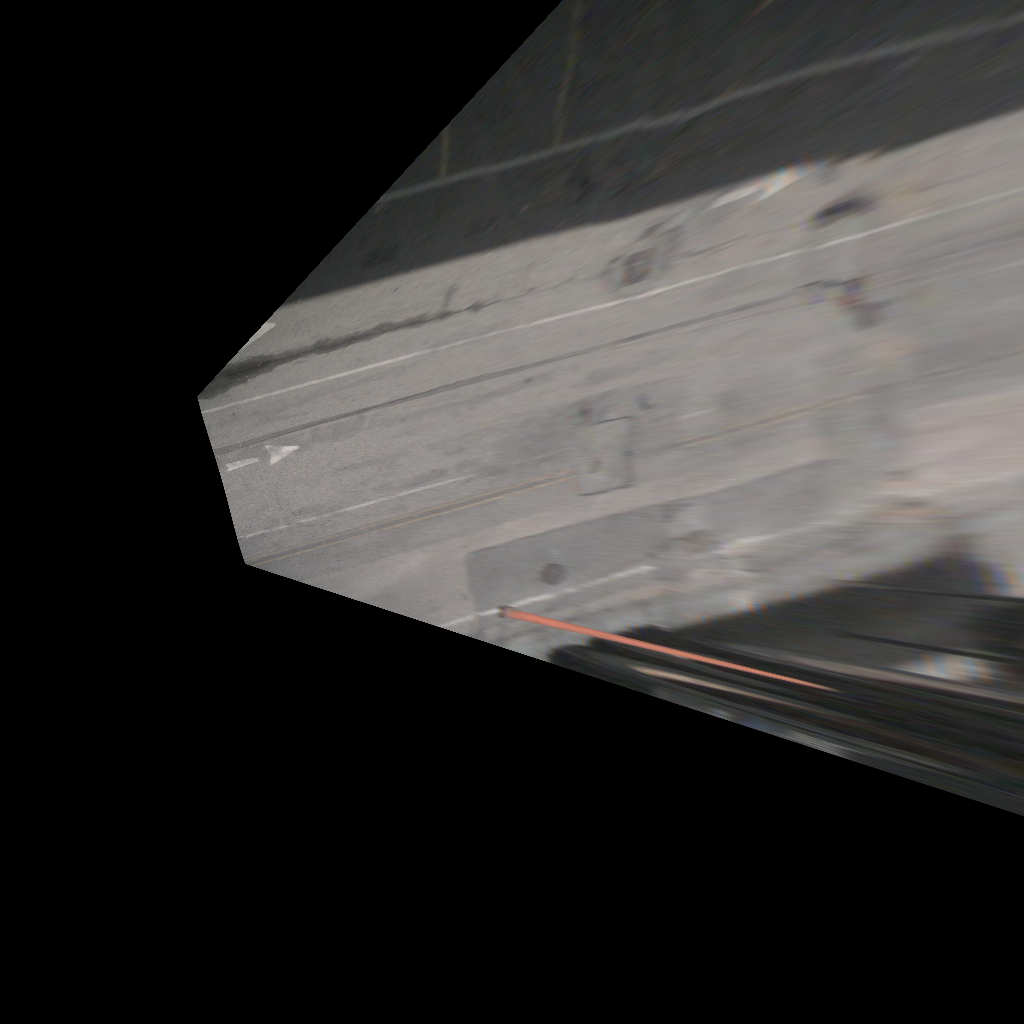
\includegraphics[width=0.15\textwidth]{images/methodology/data_augmentations/rx_0.25_4.png} \\ 
        
        \rotatebox{90}{\textbf{Pitch}} & 
        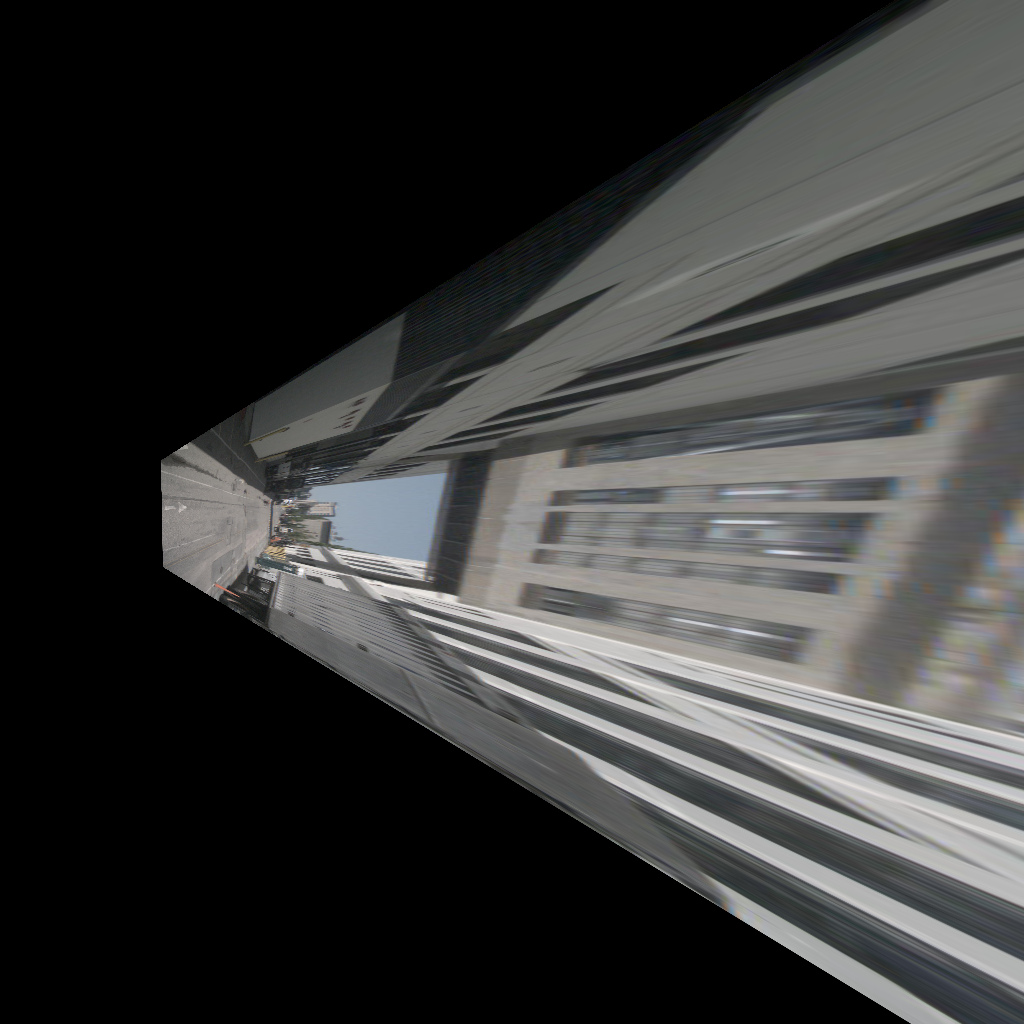
\includegraphics[width=0.15\textwidth]{images/methodology/data_augmentations/rz_-0.25_0.png} & 
        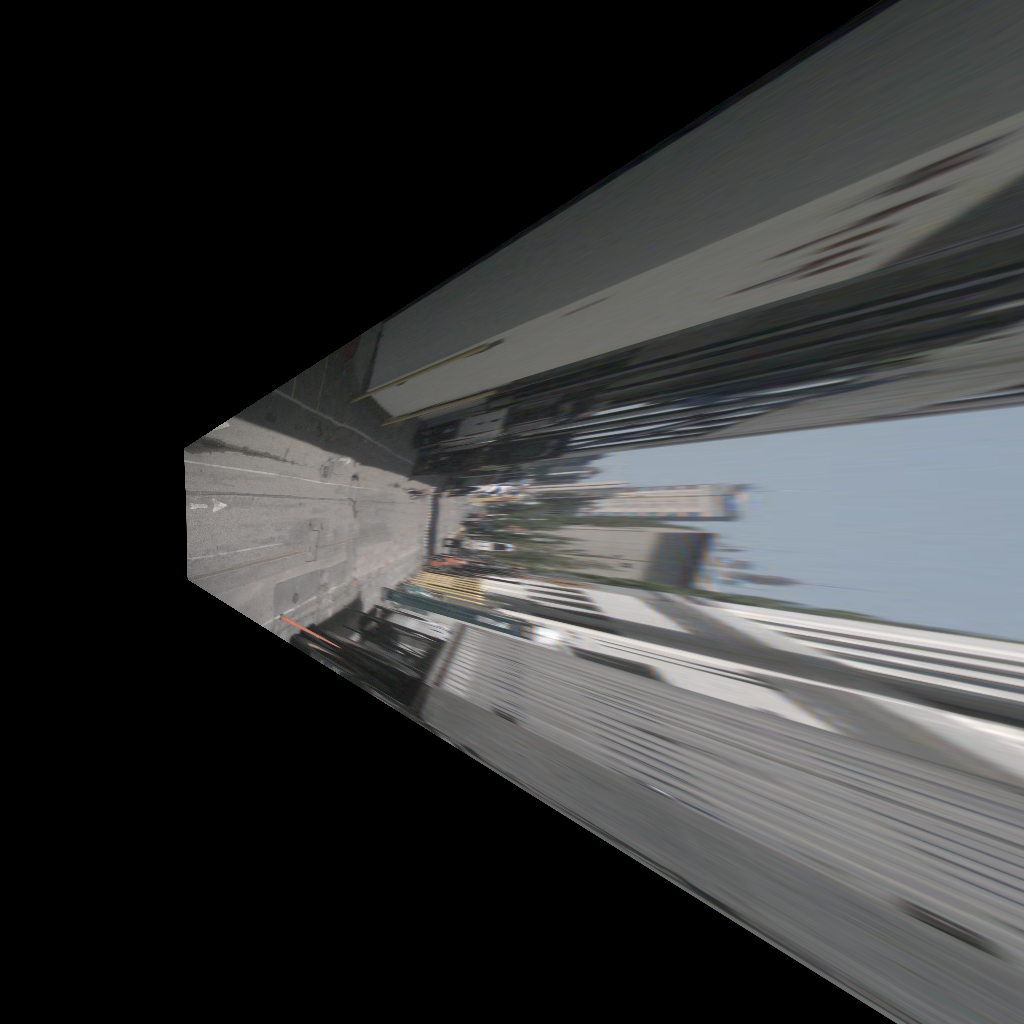
\includegraphics[width=0.15\textwidth]{images/methodology/data_augmentations/rz_-0.125_1.png} & 
        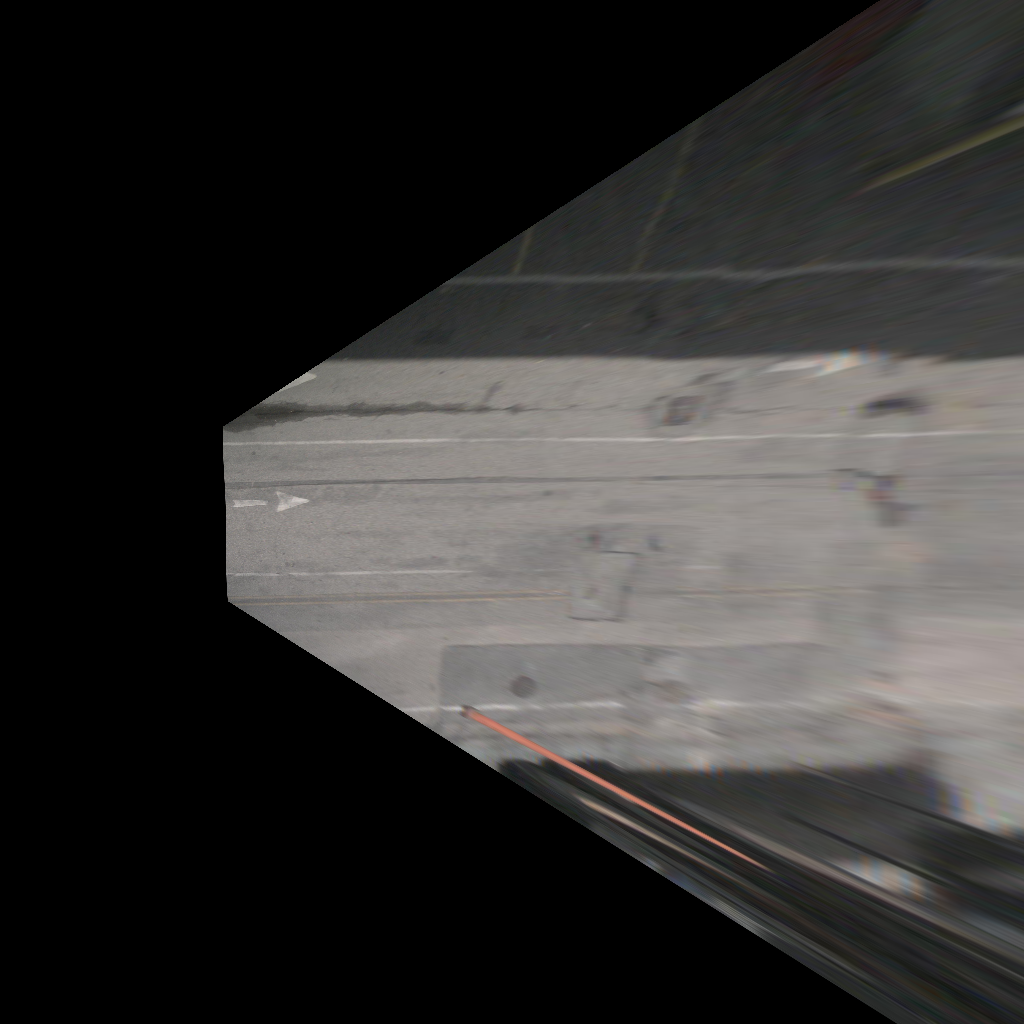
\includegraphics[width=0.15\textwidth]{images/methodology/data_augmentations/rz_0.0_2.png} & 
        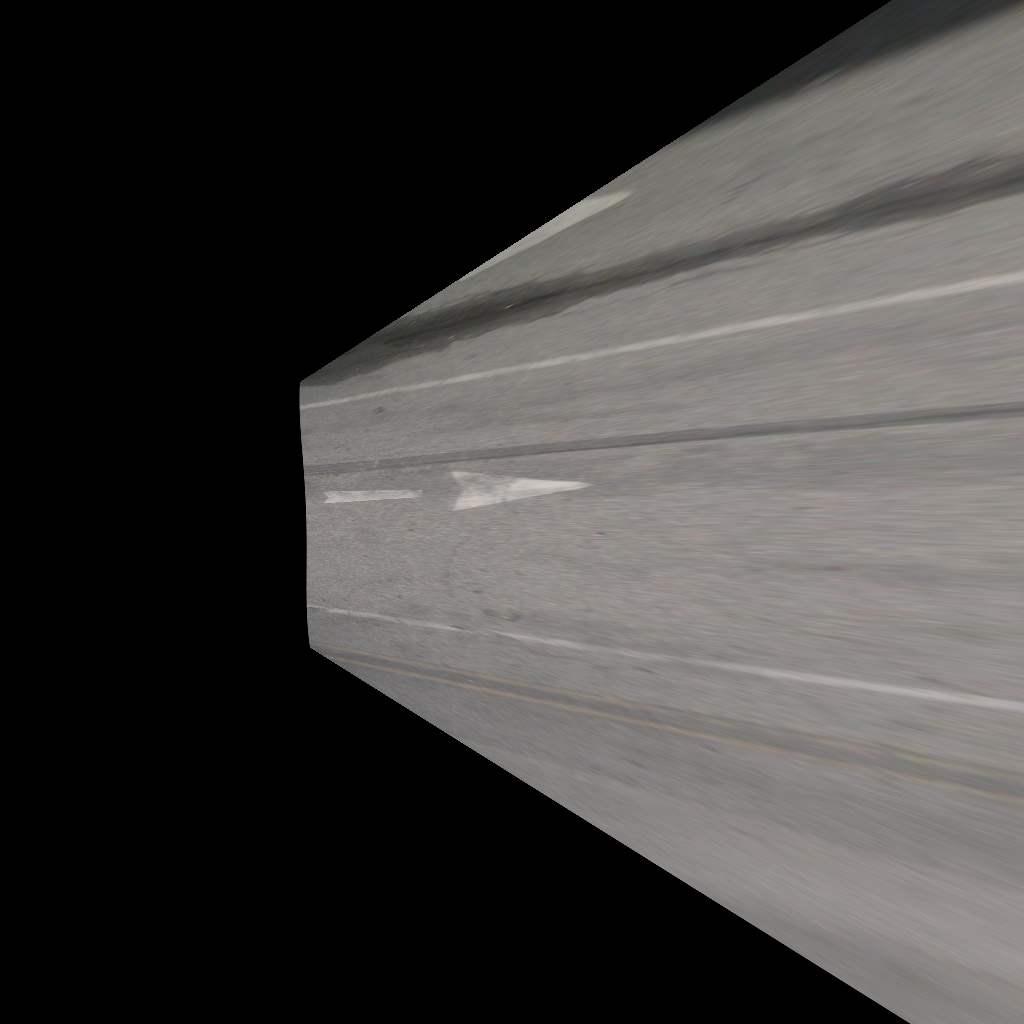
\includegraphics[width=0.15\textwidth]{images/methodology/data_augmentations/rz_0.125_3.png} & 
        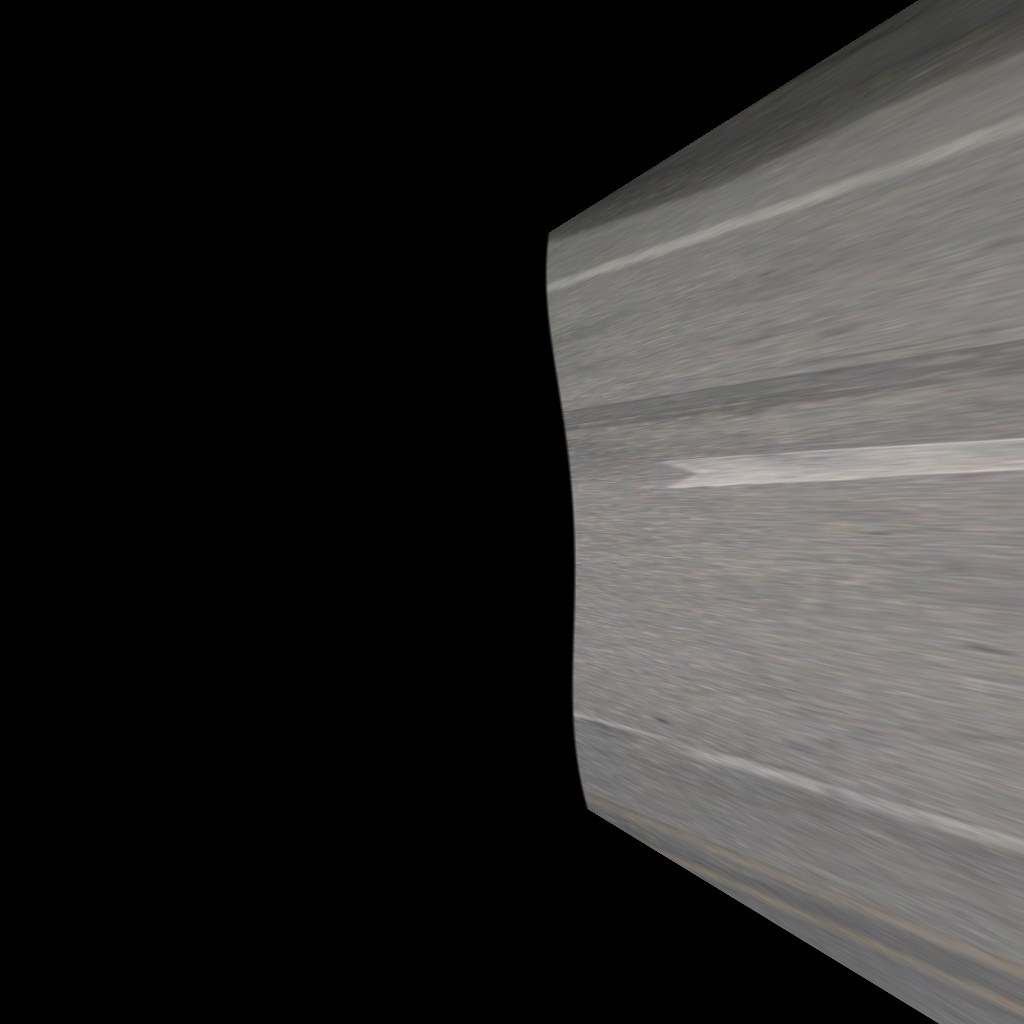
\includegraphics[width=0.15\textwidth]{images/methodology/data_augmentations/rz_0.25_4.png} \\ 

        \rotatebox{90}{\textbf{Roll}} & 
        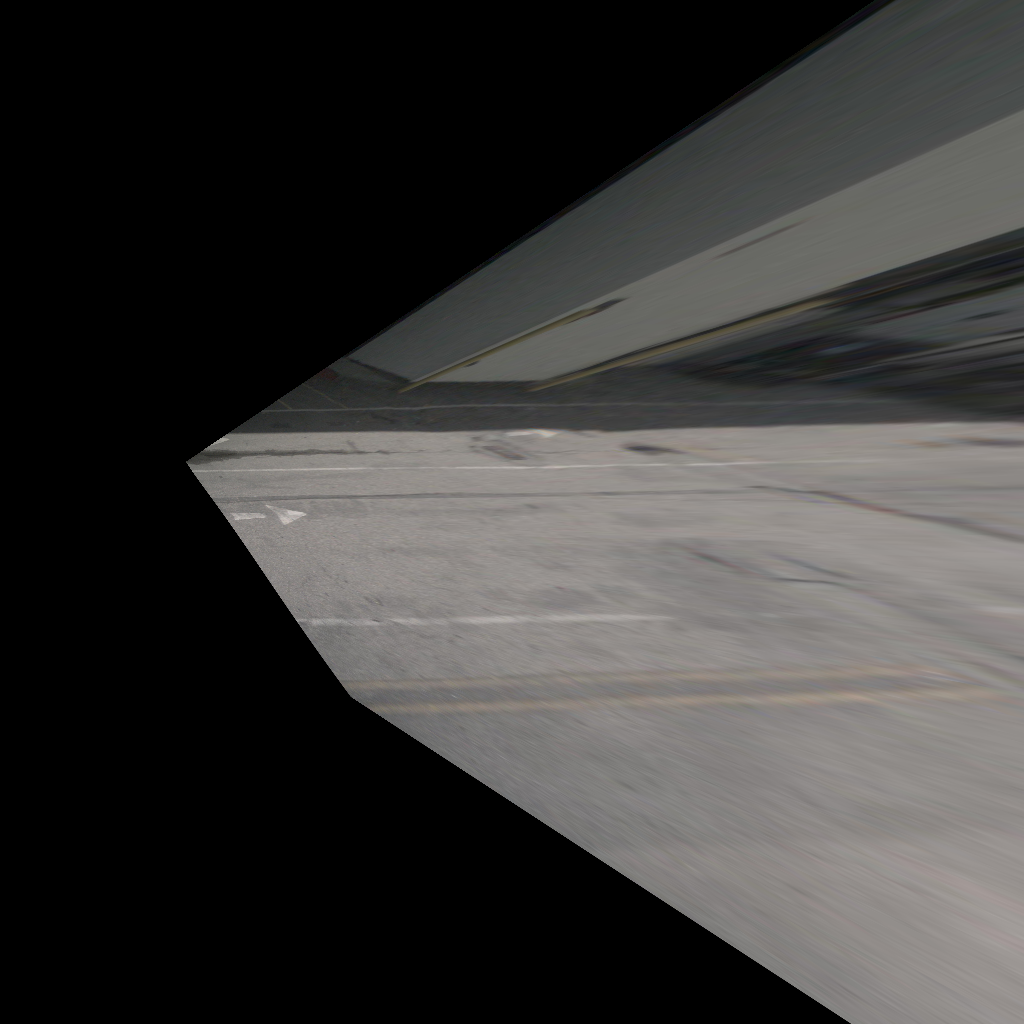
\includegraphics[width=0.15\textwidth]{images/methodology/data_augmentations/ry_-0.25_0.png} & 
        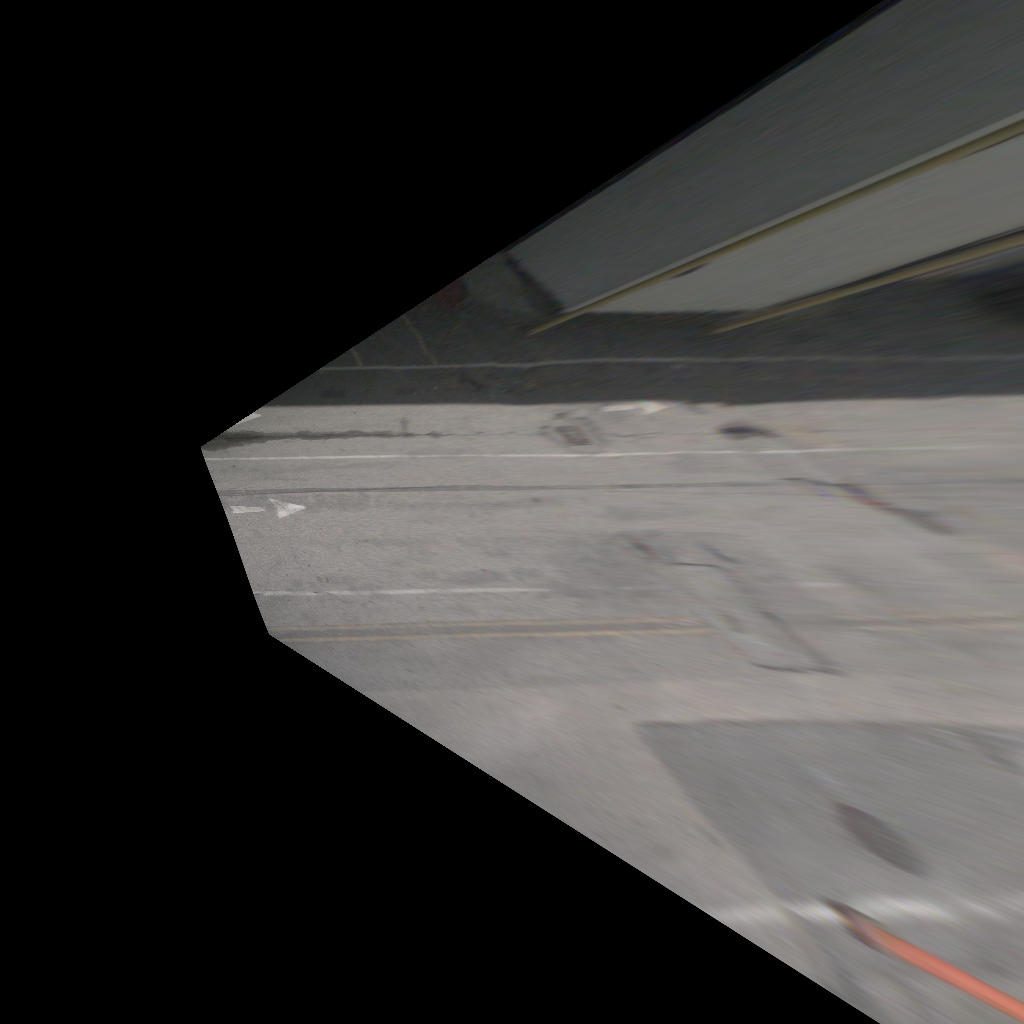
\includegraphics[width=0.15\textwidth]{images/methodology/data_augmentations/ry_-0.125_1.png} & 
        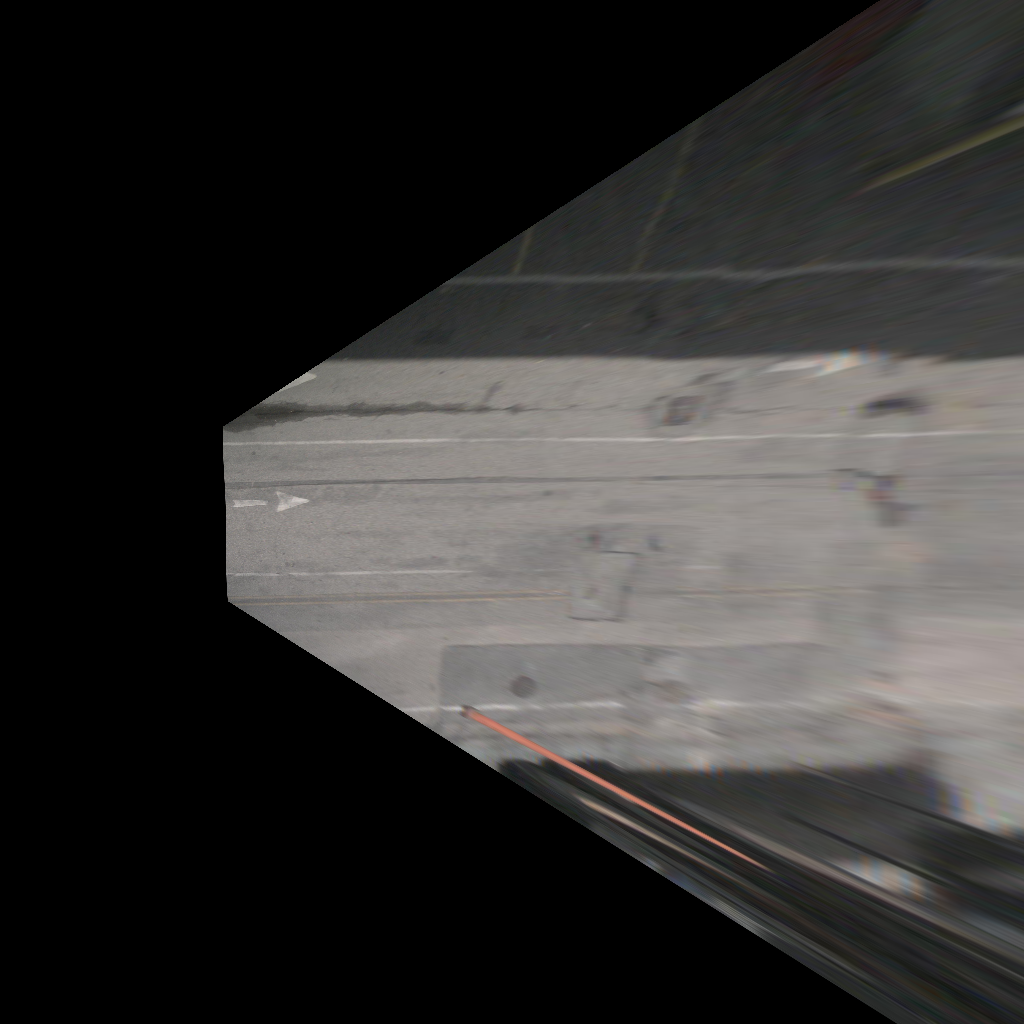
\includegraphics[width=0.15\textwidth]{images/methodology/data_augmentations/ry_0.0_2.png} & 
        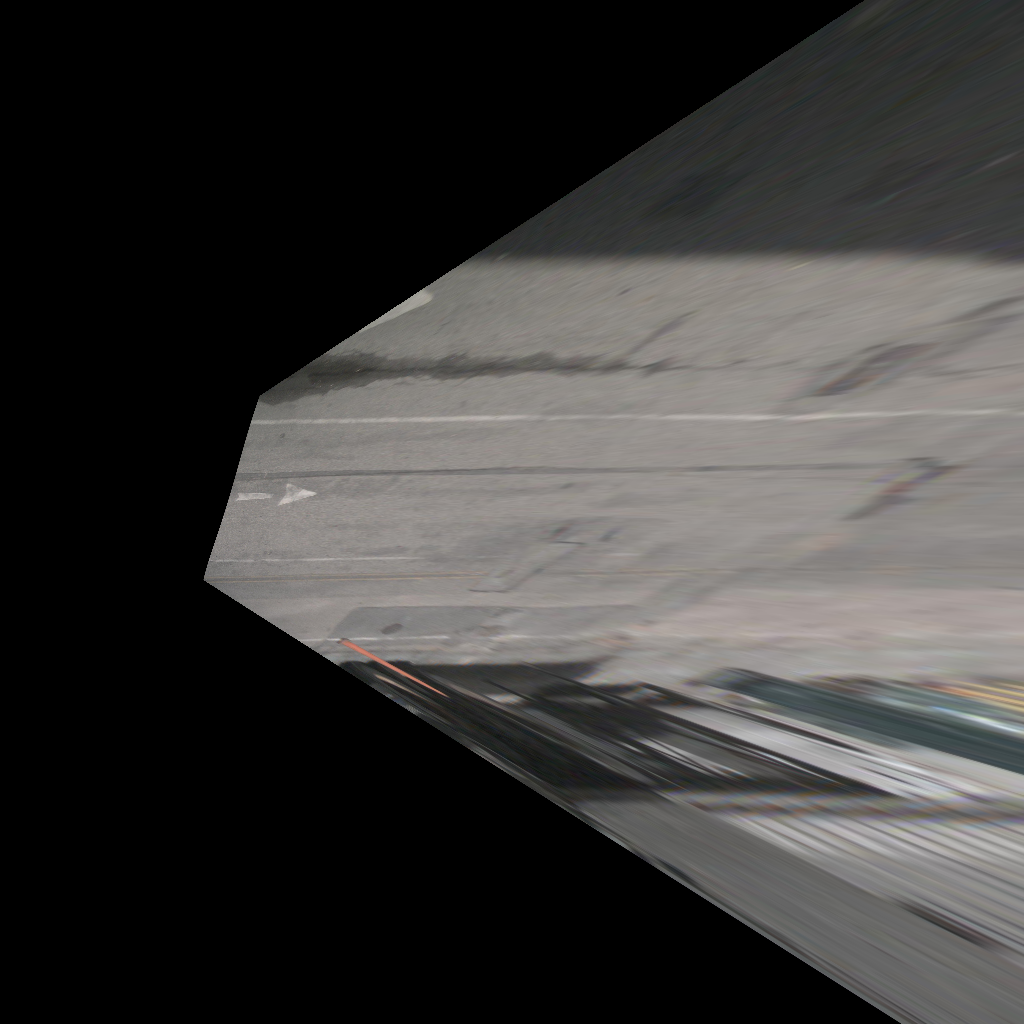
\includegraphics[width=0.15\textwidth]{images/methodology/data_augmentations/ry_0.125_3.png} & 
        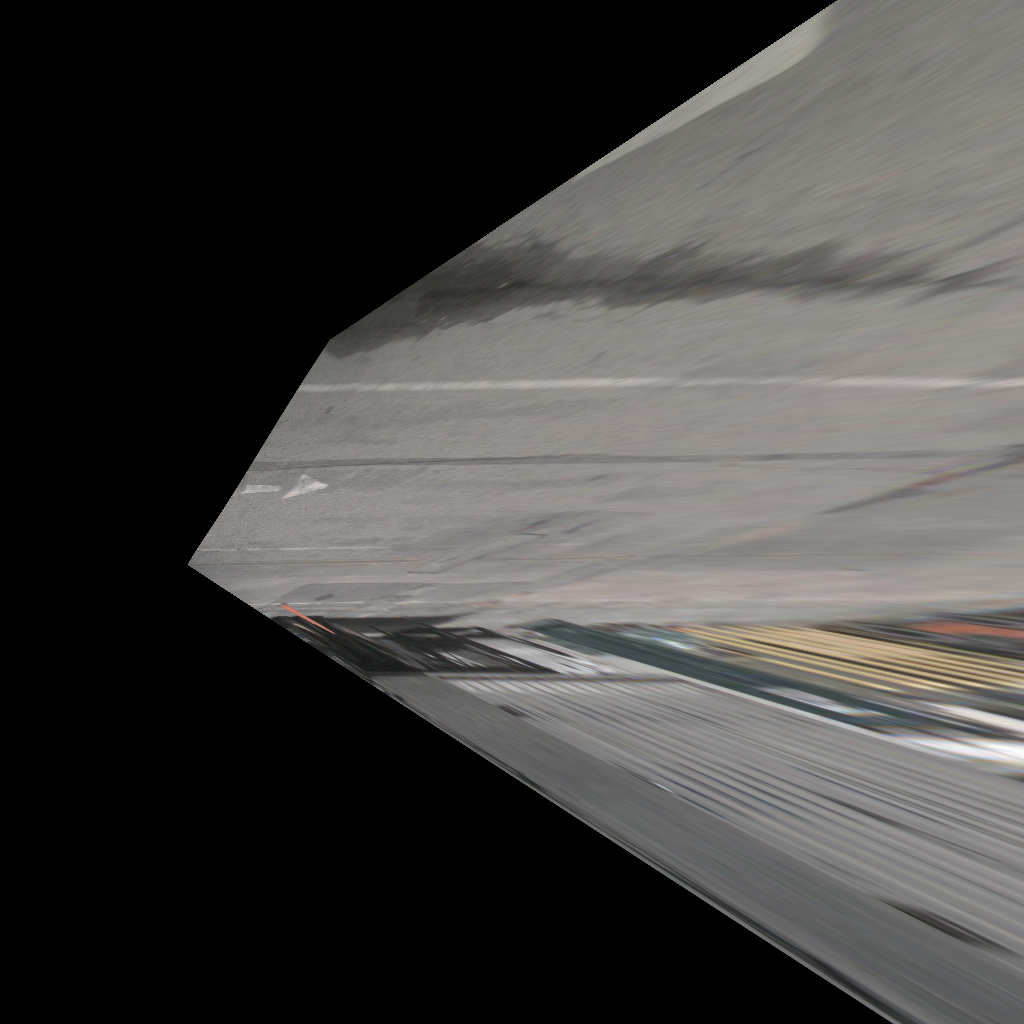
\includegraphics[width=0.15\textwidth]{images/methodology/data_augmentations/ry_0.25_4.png} \\ 
        
    \end{tabular}
    
    \caption{Effect of camera transformations on BEV projection. The first row shows variations in the yaw axes, the second in pitch, and the third in roll.}
    \label{fig:bev_data_aug}
\end{figure}


With the inclusion of random cropping, flippingf and rescaling augmentation strategies on both normal and \aclink{BEV} images, the overfitting behavior was significantly reduced as shown in Figure~\ref{fig:before_after_data_aug}.


\hl{Temporal graph!!}
\begin{figure}[h!]
    \centering
    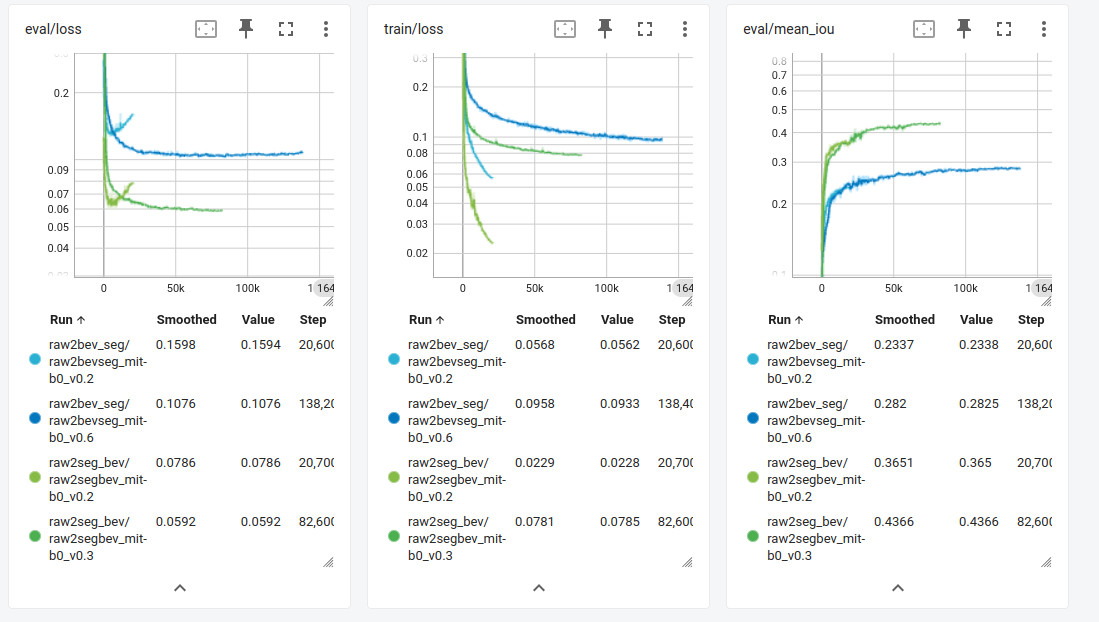
\includegraphics[width=0.7\linewidth]{./images/experiments/before_an_after_data_aug.png}
    \caption{Before and after regularization techniques. Light colors before, darker colors after. BEV segmentation model uses normal data augmentations.}
    \label{fig:before_after_data_aug}
\end{figure}


\hl{This raises an important question: \textit{Which approach is more effective: traditional geometric data augmentation techniques or the modification of extrinsic parameters?}}

\hl{Comparison between normal geometric data augmentation techniques and camera's extrinsic parameters modifications.}

The objective of this section is to show what of the data augmentation techniques is better for \aclink{BEV} semantic segmentation training and how the modification of the camera extrinsic's parameters affects the semantic predictions.

Despite significantly reducing the overfitting, normal data augmentations for \aclink{BEV} images


\subsubsection{Pipeline comparison}
\hl{raw2seg\_bev results compared with raw2bev\_seg results.}



\subsection{3D detections evaluation}
\hl{Explain the selected NuScenes selected vehicle scene, and expose the metrics used (mIoU and v2v distance).}



% ==============================================================================
Como se ha comentado anteriormente, el objetivo final del pipeline de anotación es generar máscaras de ocupación, oclusión y área conducible. Para lograrlo, se parte de máscaras semánticas del entorno tanto en el dominio de la cámara como en vista \aclink{BEV}. Un paso intermedio crucial en este proceso es la detección 3D de objetos a partir de imágenes monoculares en el dominio de la cámara, con el fin de estimar las dimensiones y posiciones de los obstáculos. Esta detección se lleva a cabo mediante algoritmos de clustering de nubes de puntos y, dado su papel central, es especialmente relevante evaluar su precisión mediante métricas adecuadas.

El dataset nuScenes fue desarrollado, entre otros fines, para facilitar el entrenamiento y la evaluación de este tipo de estrategias de percepción 3D. Este conjunto de datos incluye diversas métricas estandarizadas para medir la calidad de las detecciones. Entre ellas, destaca en primer lugar la Mean Average Precision (mAP), una métrica ampliamente utilizada para evaluar modelos de detección. El mAP se define como el área bajo la curva de precision-recall, y refleja el equilibrio entre la precisión (proporción de verdaderos positivos respecto a todas las predicciones positivas) y el recall (proporción de verdaderos positivos respecto a todos los elementos relevantes del conjunto de datos).

Para calcular el mAP, es necesario establecer previamente un criterio de correspondencia entre las predicciones y el ground truth. En muchos casos este proceso se realiza mediante la métrica de Intersection over Union (IoU), que evalúa la superposición espacial entre predicción y realidad. Si el IoU supera un determinado umbral, se considera un true positive; si no, un false positive. Las instancias del ground truth sin predicciones asociadas se consideran false negatives. En el caso de NuScenes, sin embargo, la correspondencia no se basa en el IoU, sino en la distancia 2D entre los centros de las cajas en el plano del suelo. Así, para diferentes umbrales de distancia (0.5, 1, 2 y 4 metros), se calcula la Average Precision (AP) correspondiente, y el mAP final se obtiene como la media de las APs para todas las clases y umbrales considerados.

Además del mAP, nuScenes propone un conjunto de métricas adicionales que permiten evaluar de forma más específica distintos aspectos de las detecciones correctamente clasificadas (true positives). Estas métricas cuantifican errores en distintos atributos clave del objeto detectado, utilizando un umbral fijo de 2 metros para establecer la asociación entre predicción y ground truth. Las principales métricas de este tipo son:

\begin{itemize}
    \item Average Translation Error (ATE): mide el error de traslación como la distancia euclídea entre los centros de las cajas predichas y las reales, proyectados en el plano del suelo.
    
    \item Average Scale Error (ASE): calcula el error de escala como $1 - IoU$, una vez alineadas la orientación y la posición de las cajas.
    
    \item Average Orientation Error (AOE): mide el error de orientación como la menor diferencia angular en el eje de guiñada (yaw) entre predicción y realidad.
    
    \item Average Velocity Error (AVE): representa el error absoluto en la estimación de la velocidad del objeto, medido en metros por segundo.

    \item Average Attribute Error (AAE): evalúa el error en la predicción de atributos dinámicos (por ejemplo, si un coche está aparcado, en movimiento o detenido) como $1 - acc$, siendo $acc$ el accuracy o la proporción de aciertos en la clasificación del atributo.
\end{itemize}

Como métrica global, NuScenes propone el NuScenes Detection Score (NDS), que sintetiza la calidad general de las detecciones mediante una combinación ponderada de todas las métricas anteriores. Esta métrica permite obtener una visión de conjunto del rendimiento del sistema, equilibrando precisión, localización, orientación, velocidad, escala y atributos.

El caso de uso abordado en este trabajo presenta particularidades que lo diferencian del escenario estándar planteado en el dataset NuScenes. En concreto, las detecciones 3D se obtienen a partir de imágenes monoculares mediante algoritmos de clustering, por lo que los cuboides 3D generados únicamente representan la parte visible del objeto desde la cámara en un instante determinado. Además, estos cuboides están siempre alineados con la orientación de la cámara, lo que hace que el cálculo del error de orientación carezca de utilidad práctica en este contexto, ya que se sabe de antemano que este error será elevado. No obstante, resulta de gran interés evaluar la precisión en la estimación de las posiciones y dimensiones de los cuboides generados, ya que ello permite valorar si el pipeline es capaz de realizar detecciones razonablemente precisas con la información disponible.

En este escenario, emplear la distancia entre centroides como criterio de asociación entre predicciones y ground truth resulta problemático. Mientras que los cuboides del ground truth engloban la totalidad del objeto en 3D, los cuboides predichos solo contienen los puntos visibles desde la cámara, lo que genera desplazamientos sistemáticos en las posiciones relativas de los centros. Por ello, se ha optado por utilizar una métrica más adecuada: la distancia entre volúmenes (volume-to-volume distance, o v2v), definida como la distancia mínima entre las envolventes convexas de los volúmenes considerados.

Sin embargo, la métrica v2v presenta una limitación importante: toma un valor de cero siempre que exista intersección entre los volúmenes, independientemente del grado de solapamiento. Para superar esta limitación se recurre a la métrica Bounding Box Disparity (BBD) [referencia], que combina IoU y v2v en una única métrica continua y no negativa. Esta métrica permite cuantificar la disimilitud entre dos cuboides, tanto si se solapan como si no. Como se indica en la definición original, mientras que el IoU únicamente puede comparar cuboides con intersección, el BBD proporciona una medida de disparidad también en ausencia de solapamiento. Su interpretación es la siguiente:

\begin{itemize}
    \item Si $BBD = 0$, los cuboides son idénticos (intersección total).
    \item Si $0 < BBD < 1$, existe solapamiento pero también disparidad.
    \item Si $BBD \geq 1$, los cuboides no se solapan.
\end{itemize}

Estos distintos casos se ilustran en la Figura X.

Por otra parte, para evaluar el error en la estimación de las dimensiones de los objetos detectados, se ha decidido calcular la diferencia absoluta entre las dimensiones de los cuboides predichos y del ground truth en cada uno de los ejes (longitud, anchura y altura). Esto permite analizar en qué dimensión se concentra mayor error y bajo qué condiciones.

El proceso de evaluación comienza delimitando el área en la que se considerarán las detecciones generadas por el pipeline. Dado que el sistema produce predicciones a distancias mayores que las empleadas posteriormente para generar las máscaras BEV de ocupación y oclusión, se ha decidido restringir el rango de evaluación a la misma región que se usa para la generación de dichas máscaras. Concretamente, se define el polígono de visión de la cámara proyectado sobre el plano horizontal y se limita la distancia máxima de detección a 15 metros. De este modo, solo se consideran para la evaluación aquellas detecciones y elementos del ground truth que se encuentren dentro de este polígono en el instante correspondiente.

Una vez filtradas las detecciones, se procede a la asociación entre predicciones y ground truth mediante la resolución del Linear Sum Assignment Problem (LSAP) utilizando el algoritmo húngaro. Esto permite encontrar las correspondencias óptimas entre objetos predichos y reales, sobre las cuales se calculan las siguientes métricas:

\begin{itemize}
    
    \item True Positives (TP), False Positives (FP) y False Negatives (FN): determinados en función de las asociaciones establecidas.
    
    \item DD (Difference in Dimensions): diferencia de volumen entre cuboides asociados.

    \item DED (Difference in Each Dimension): diferencia absoluta por eje (longitud, anchura, altura).
    
    \item v2v: distancia entre volúmenes.

    \item IoU: intersección sobre unión en 3D.
    
    \item BBD (Bounding Box Disparity): métrica continua de disimilitud explicada anteriormente.
\end{itemize}
    
Estas métricas permiten evaluar de manera más precisa y adaptada la calidad de las detecciones 3D en el contexto particular del pipeline propuesto, considerando las limitaciones y características propias del proceso de detección monocular.
% ==============================================================================

\begin{figure}[h]
    \centering
    % Row labels
    \setlength{\tabcolsep}{1pt}  % Reduce column padding
    \renewcommand{\arraystretch}{0.5}
    \begin{tabular}{c c}
        
        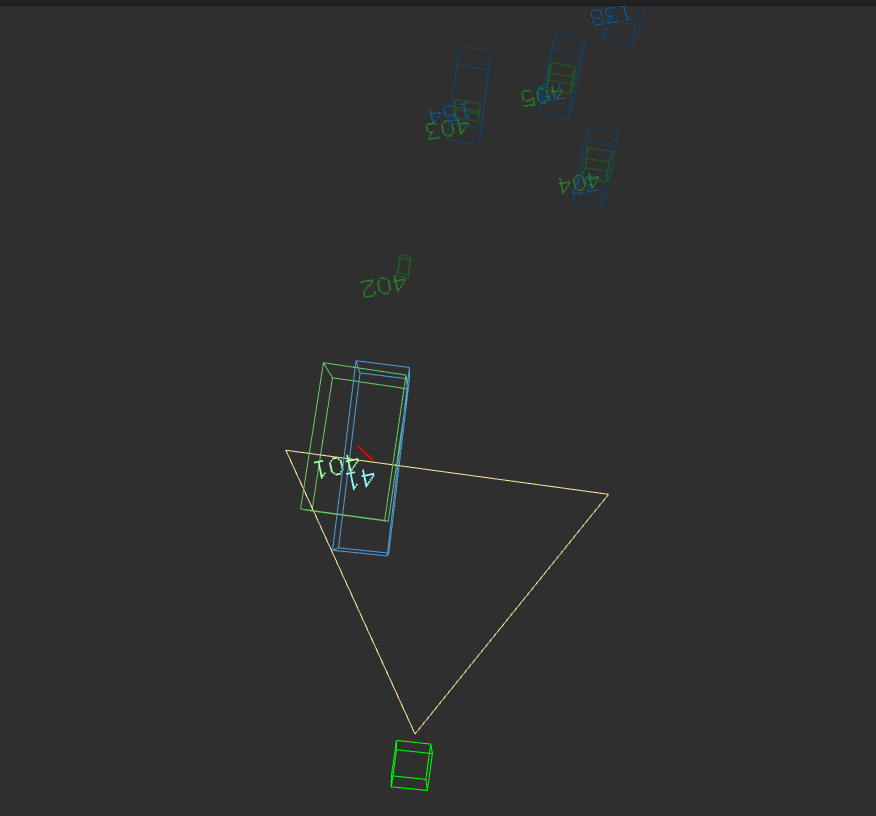
\includegraphics[width=0.45\textwidth]{images/experiments/frame_0_3d_scene.png} &
        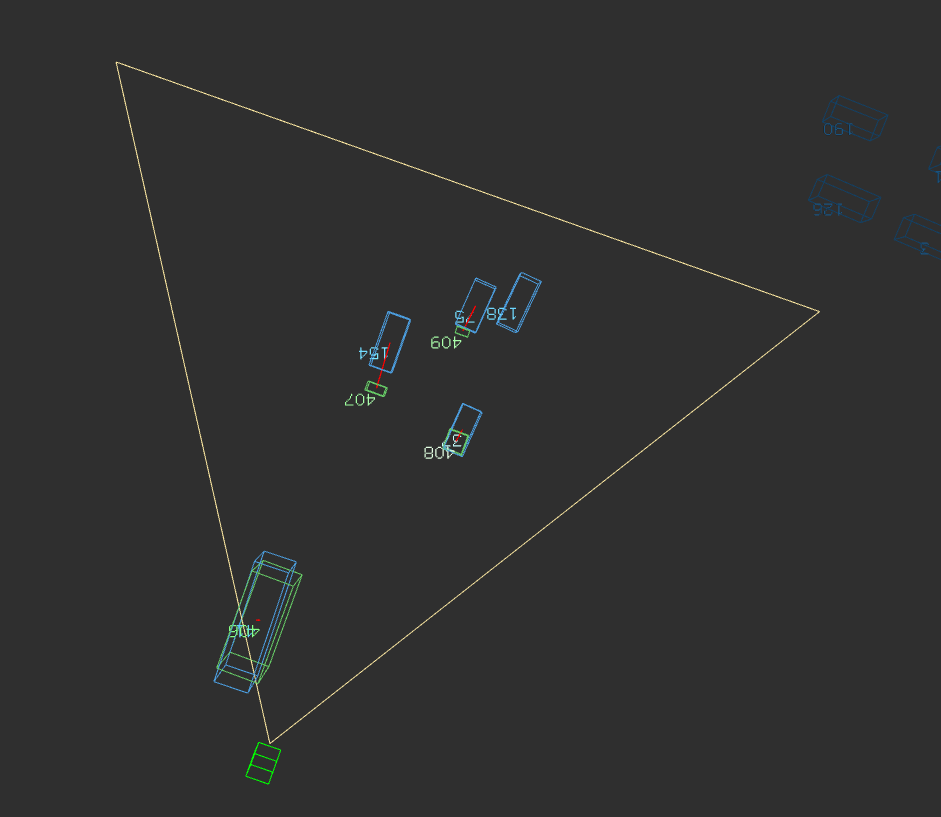
\includegraphics[width=0.45\textwidth]{images/experiments/frame_2_3d_scene.png} \\
        
        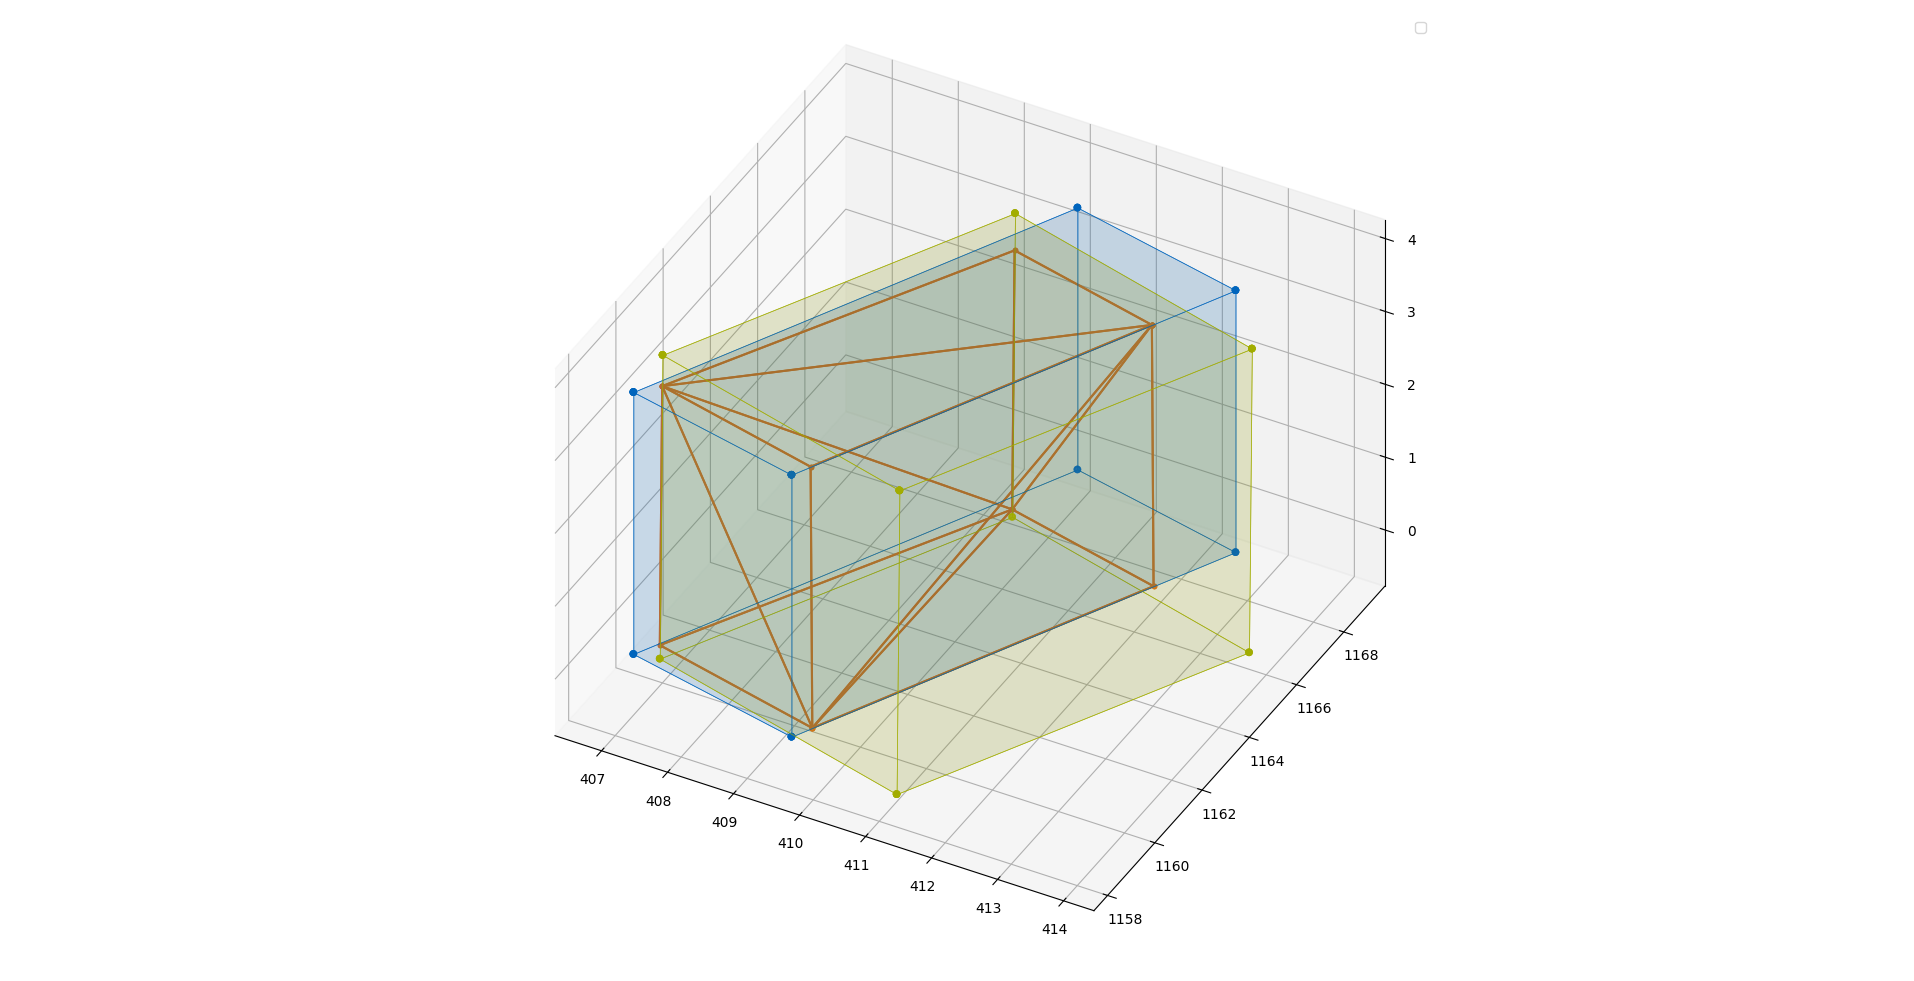
\includegraphics[width=0.45\textwidth]{images/experiments/frame_0_3d_bb.png} &
        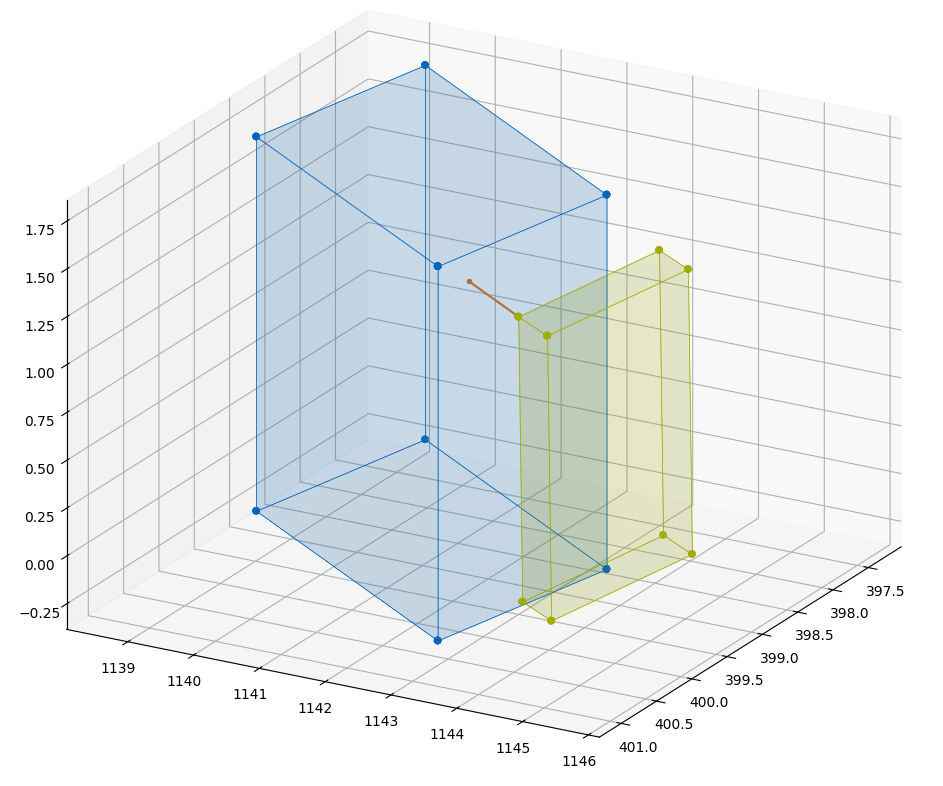
\includegraphics[width=0.45\textwidth]{images/experiments/frame_2_3d_bb.png} \\

    \end{tabular}
    
    \caption{Bounding Box Disparity scene calculation. (a) shows an example of intersection, while (b) shows an example of volumetric distance}
    \label{fig:bbox_disparity}
\end{figure}


\subsection{BEV masks evaluation}
\hl{Groundtruth BEV masks could be generated from annotations and compute mIoU between the annotated BEV masks and ground truth ones.}

